\chapter{SOIL WATER BALANCE}

Plant production involves intake of atmospheric CO$_{{\rm 2}}$ through stomatal openings in the
epidermis. Most of the water that plants take up from the soil is again lost to the
atmosphere by transpiration through the same openings. The daily turnover can be
considerable: transpiration from 0.4 cm of water from a crop surface on a clear sunny
day corresponds with a water loss from the root zone of than 40.000 kg ha$^{{\rm -1}}$ 
d$^{{\rm -1}}$. If soil
moisture take up by the roots is not replenished, the soil will dry out to such an extent
that the plants wilt and - ultimately - die.

The tenacity with which the soil retains its water is equaled by the suction which the
roots must exert to be able to take up soil moisture. This suction known as the soil
moisture potential or 'matrix suction', can be measured. In hydrology, the potential is
usually used and is expressed as energy unit per weight of soil water, with the dimension
of length (van Bakel, 1981). An optimum range exists within which the plant takes up
water freely. Above or below this level the plant senses stress. It reacts by actively
curbing its daily water consumption through partial or complete closure of the stomata.
The consequence is evident: this stomatal closure interferes with CO$_{{\rm 2}}$ intake and 
reduces assimilation and, consequently, dry matter production.

A crop growth simulation model must therefore keep track of the soil moisture potential
to determine when and to what degree a crop is exposed to water stress. This is common\-ly 
done with the aid of a water balance equation, which compares for a given period of
time, incoming water in the rooted soil with outgoing water and quantifies the difference
between the two as a change in the amount of soil moisture stored.

Therefore the purpose of the soil water balance calculations is to estimate the daily value
of the actual soil moisture content, which influences soil moisture uptake and crop
transpiration.

\begin{figure}[p]
%Fig. 6.1
\centering
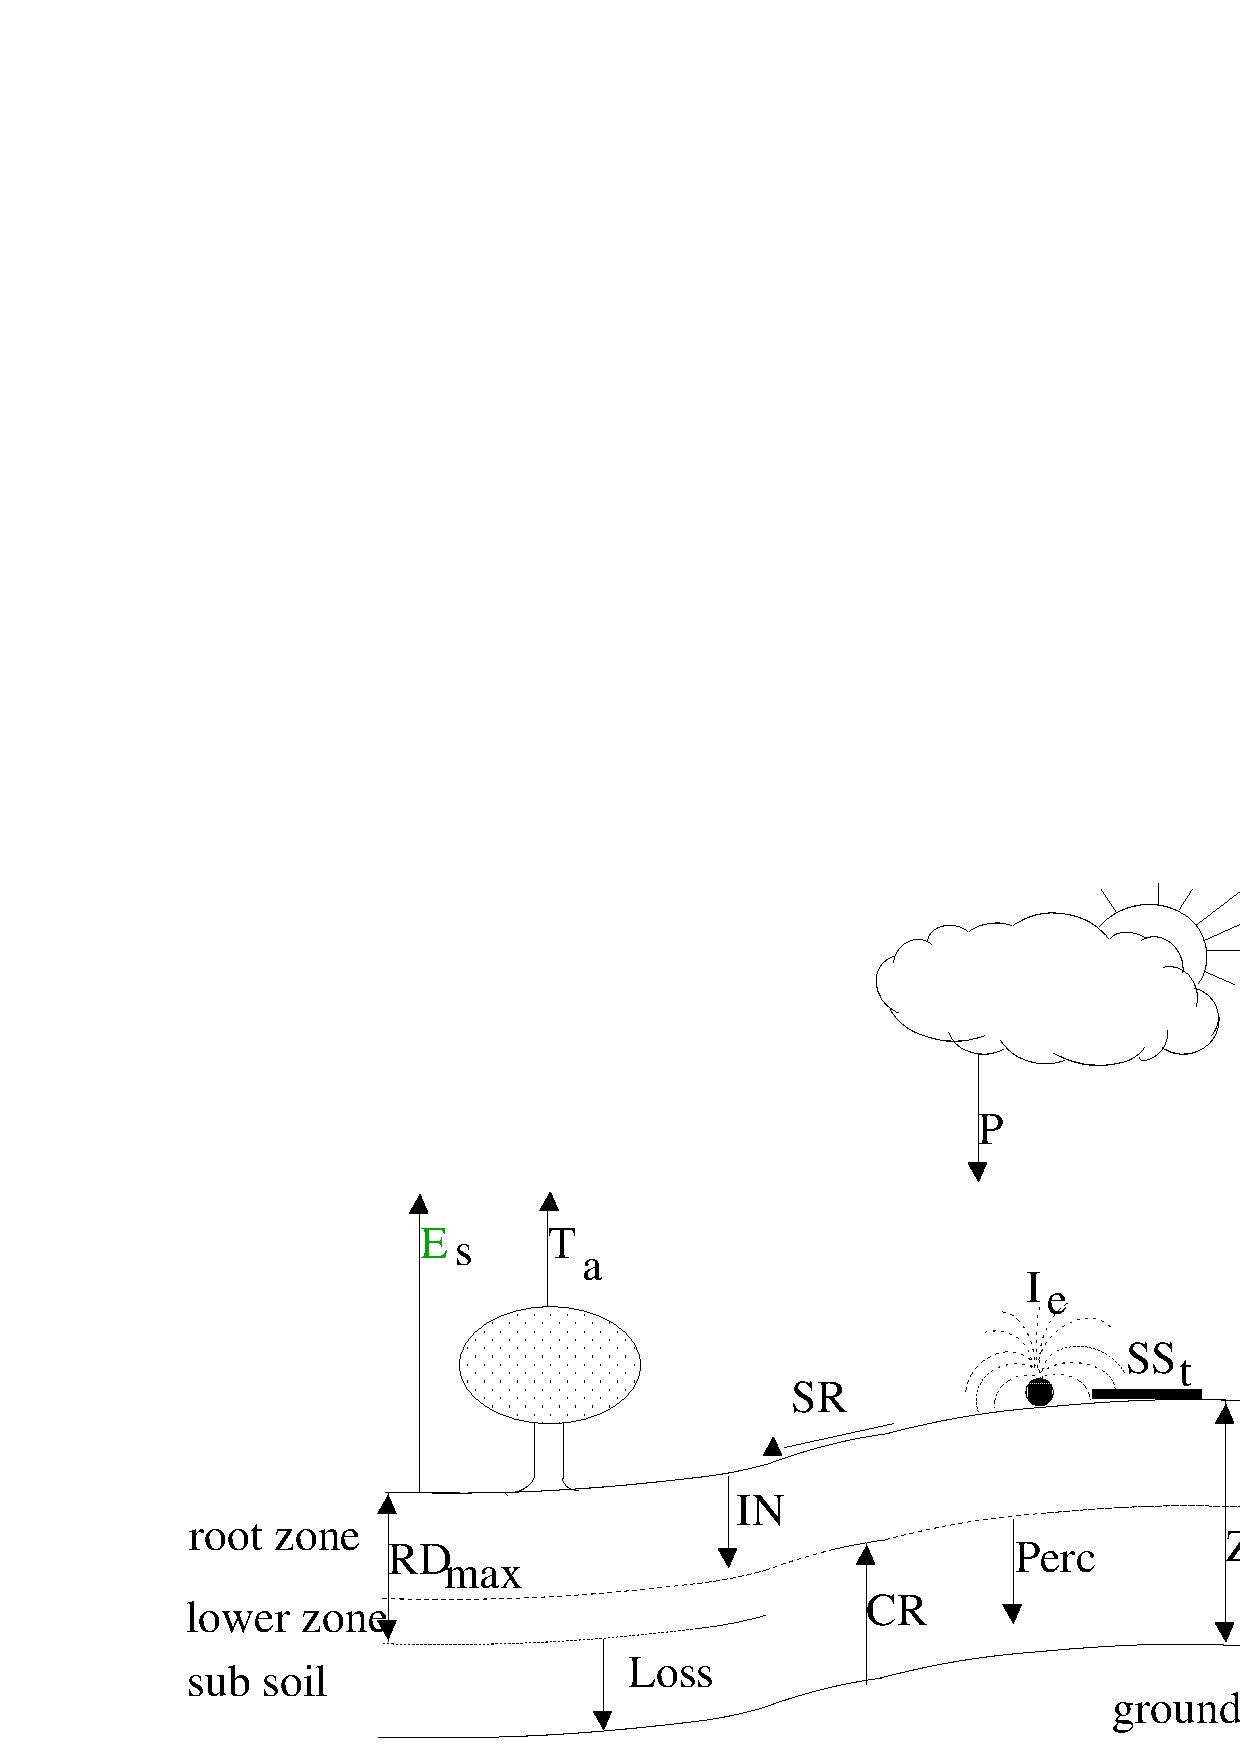
\includegraphics[width=120mm]{\FigDir/WATBAL1.pdf}
\caption{Sche\-matic repre\-senta\-tion of the differ\-ent compo\-nents of a soil water balance}
\label{fig:WatBalSchematic}
\end{figure}
The actual soil moisture content can be established according to (Driessen, 1986):

\begin{align}
% equations 6.1a-b
\theta_{t~}   = {\frac{IN _{up} ~+~(IN _{low} ~-~T _{a} )}{RD}} \Delta t \subeqn  \\
where IN_{up} = P~+~I _{e} ~-~E _{s} ~+~SS _{t} \, /\Delta t-~SR  \subeqn  \\
and IN_{low} = CR~-~Perc \subeqn \\
\end{align}

Where:\\
\begin{tabularx}{\textwidth}{llXr}
$\theta$$_{{\rm t}}$ &:& Actual moisture content of the root zone at time step t   & [cm$^{{\rm 3}}$ cm$^{{\rm -3}}$]\\
IN$_{{\rm up}}$ &:& Rate of net influx through the upper root zone boundary  & [cm d$^{{\rm -1}}$]\\
IN$_{{\rm lo}}$$_{{\rm w}}$ &:& Rate of net influx through the lower root zone boundary  & [cm d$^{{\rm -1}}$]\\
T$_{{\rm a}}$ &:& Actual transpiration rate of crop   & [cm d$^{{\rm -1}}$]\\
RD &:& Actual rooting depth  & [cm]\\
P &:& Precipitation intensity  & [cm d$^{{\rm -1}}$]\\
I$_{{\rm e}}$ &:& Effective daily irrigation  & [cm d$^{{\rm -1}}$]\\
E$_{{\rm s}}$ &:& Soil evaporation rate   & [cm d$^{{\rm -1}}$]\\
SS$_{{\rm t}}$ &:& Surface storage  & [cm]\\
SR &:& Rate of surface runoff  & [cm d$^{{\rm -1}}$]\\
CR &:& Rate of capillary rise  & [cm d$^{{\rm -1}}$]\\
Perc &:& Percolation rate  & [cm d$^{{\rm -1}}$]\\
$\Delta$t &:& Time step  & [d]\\
Z$_{{\rm t}}$ &:& Depth of groundwater table (see figure 6.1)  & [cm]\\
\end{tabularx}

Processes directly affecting soil moisture content of the root zone can be defined as:
\begin{itemize}
\item infiltration is transport from the soil surface into the root zone;
\item evaporation is the loss of soil moisture to the atmosphere;
\item transpiration by plants is loss of water from the interior root zone;
\item percolation is downward transport of water from the root zone to the layer below the root zone;
\item capillary rise is upward transport into the rooted zone.
\end{itemize}

The water balance equation has to be solved for each time interval in the crop growth cycle.

In the model the soil water balance calculations for potential production and the soil water
balance calculations for water limited production have been separated into different
subroutines. For the calculation of potential production the soil moisture content is
assumed to be at field capacity and no calculations have to be performed to simulate the
water balance in the soil. Only the actual evaporation rate and the actual transpiration rate
have to be accumulated. 

For the calculation of the water limited production two different soil water balances are
distinguished. One soil water balance without groundwater influence (i.e. for a freely
draining soil) and one soil water balance with groundwater influence. In the JRC version
of WOFOST, the system with groundwater is not activated because of lack of sufficiently
good data. However, the groundwater option can be easily applied whenever data are
made available.So, actually three water balance subroutines can be distinguished:
\begin{itemize}
\item Potential production [WATPP, \S  6.2]\\
\item Water limited production, without groundwater influence [WATFD, \S  6.3]\\
\item Water limited production, with groundwater influence [WATGW, \S  6.4]
\end{itemize}
 
The actual transpiration rate of a canopy, used in the calculations of potential and water
limited production, is calculated in the same way for all options. The calculation method
will therefore be treated separately in \S 6.1. 

The capillary rise in the system with groundwater influence is a complicated subject. It
will be discussed separately in \S 6.5.

In the calculations for the water limited growth the water content of the root zone is the
most important state variable. In- and outflow of water is calculated for each time step. It
is important to realize that the model is not intended for detailed physical treatment of
water movement in the soil, but only for estimating moisture availability to the crop. The
distribution of water within the root zone is assumed to be instan\-taneous (within the time
step of the model, being one day). The available water contained in the rooted zone is
directly at the disposal of the crop. Water just below the root zone is available after
further root growth and water below the potential rooting depth cannot be used by the
crop.

The process of infiltration is not treated in a physical sense at all, because simulation of
this process would require a much smaller time step (Rietveld, 1978; Stroosnijder {\it et al\/}.,
1972; van Keulen \& van Beek, 1971). Instead a predefined fraction of the rain is not
infiltrating on the day of rainfall (van Diepen {\it et al\/}., 1988).

Soil water content at saturation is equal to soil porosity. Field capacity is the volumetric
water content of the soil after wetting and initial redistribution (Veihmeyer \& Hendrick\-son, 
1931). It is often treated as a soil characteristic (van Keulen, 1975; Driessen, 1986;
Jansen \& Gosseye, 1986), although it also depends on boundary conditions. Field capacity
is usually defined as the volumetric  water content at a soil moisture suction of 100 mbar
or pF 2.0 at least in the Netherlands. It is the moisture suction in equilibrium with a
groundwater table at 100 cm. Elsewhere in the world, for loamy soils field capacity
corresponds with a value of 200 mbar moisture suction. For sandy soils 60 mbar is a
realistic value under field conditions. Above a certain value of moisture suction, plants do
not recover and wilt permanently. The volumetric water content of the soil at this point is
called wilting point. The soil moisture at wilting point has usually a value of about 16000
mbar or pF 4.2. The soil moisture content of an air dry soil is assumed to be at pF 7.0
(van Keulen, 1975).

\section{Evapo(transpi)ration}

In the subroutine {\bf EVTRA} the following processes are calculated for a given crop cover:
\begin{itemize}
\item The maximum evaporation rate from a shaded soil surface;
\item The maximum evaporation rate from a shaded water surface;
\item The maximum crop transpiration rate;
\item The actual crop transpiration rate. 
\end{itemize}

Transpiration, or the rate of water loss from the plants depends on the energy available
for vaporization, on the difference in vapor pressure between the plant and the surround\-ing 
air and on the resistance to water vapor diffusion from the stomatal cavity to the
atmosphere (van Keulen \& Seligman, 1987). Potential transpiration is the water loss from
a field crop which covers the soil completely and has an optimum supply of water from
the soil. The method, introduced by Penman (1956, 1948) and for the present use,
adapted according to Choisnel {\it et al\/}. (1992), is now used for daily totals of canopy
transpiration and for daily totals of soil evaporation (Jarvis, 1981; Feddes {\it et al\/}., 1978;
van Keulen, 1975)

\subsection{Evaporation and transpiration}
Potential evapotranspiration of a crop ET0 is the sum of potential transpiration T$_{{\rm m}}$ and
soil evaporation E0$_{{\rm s}}$.

\begin{equation}
% eq 6.2
ET0 ~=~ E0_{s} ~+~ T_{m} 
\end{equation}
 
Where:\\
\begin{tabularx}{\textwidth}{llXr}
ET0 &:& Potential evapotranspiration rate (see \S 4.1.3) & [cm d$^{{\rm -1}}$]\\
E0$_{{\rm s}}$ &:& Potential evaporation of a bare soil (see \S 4.1.3)  & [cm d$^{{\rm -1}}$]\\
T$_{{\rm m}}$ &:& Maximum crop transpiration rate (see eq. 6.4)  & [cm d$^{{\rm -1}}$]\\
\end{tabularx}

For some crops the potential evapotranspiration can be higher than the Penman evapotran\-spiration. 
Therefore, in the model a correction factor, a so called  crop coefficient
(acronym: {\bf CFET}) is introduced to account for this effect. The Penman evapotranspiration
should be multiplied by this crop coefficient (Feddes, 1978; Doorenbos \& Pruitt, 1977).
The evaporation is reduced due to the presence of vegetation, which intercepts the solar
energy and reduces the windspeed. The evaporation of the soil as a function of the leaf
area index (Goudriaan, 1977; Ritchie, 1972; 1971) can be estimated as:

\begin{equation}
% eq 6.3
E0 _{s} ~=~ ET0 ~e ^{-\kappa_{gb} \, LAI}
\end{equation}

Where:\\
\begin{tabularx}{\textwidth}{llXr}
E0$_{{\rm s}}$ &:& Potential bare soil evaporation  & [cm d$^{{\rm -1}}$]\\
 $\kappa$$_{{\rm gb}}$ &:& Extinction coefficient for global radiation  & [-]\\
 LAI &:& Leaf area index  & [ha ha$^{{\rm -1}}$]\\
\end{tabularx}
 
The potential transpiration rate can be calculated by combining equations 6.2 and 6.3.

\begin{equation}
% eq 6.4
T _{m} ~=~ ET0\, (1~-~e ^{-\kappa _{gb} \, LAI} )
\end{equation}
 
Where:\\
\begin{tabularx}{\textwidth}{llXr}
T$_{{\rm m}}$ &:& Maximum crop transpiration rate & [cm d$^{{\rm -1}}$]\\
ET0 &:& Potential evapotranspiration rate & [cm d$^{{\rm -1}}$]\\
$\kappa$$_{{\rm gb}}$ &:& Extinction coefficient for global radiation & [-]\\
LAI &:& Leaf area index (see \S 5.4.5) & [ha ha$^{{\rm -1}}$]\\
\end{tabularx}

The extinction coefficient for global radiation can be estimated as a factor times the
extinction coefficient of diffuse radiation:

\begin{equation}
% eq 6.5
\kappa_{gb} ~=~ 0.75\, \kappa_{df} 
\end{equation}

Where:\\
\begin{tabularx}{\textwidth}{llXr}
$\kappa_{{\rm gb}}$ &:& Extinction coefficient for global radiation & [-]\\
$\kappa_{{\rm df}}$ &:& Extinction coefficient for diffuse light & [-]\\
\end{tabularx}

The maximum evaporation rate from a shaded water surface can be calculated in the same
way as equation 6.4: 

\begin{equation}
% eq 6.6
E _{w,\max } ~=~ E0 _{w} \,\,\, e ^{-\kappa  _{gb} LAI}
\end{equation}

Where:\\
\begin{tabularx}{\textwidth}{llXr}
E$_{{\rm w,max}}$ &:& Maximum evaporation rate from a shaded water surface & [cm d$^{{\rm -1}}$]\\
E0$_{{\rm w}}$ &:& Potential evaporation rate from a water surface (see \S 4.1.3) & [cm d$^{{\rm -1}}$]\\
$\kappa$$_{{\rm gb}}$ &:& Extinction coefficient for global radiation & [-]\\
LAI &:& Leaf area index & [ha ha$^{{\rm -1}}$]\\
\end{tabularx}

The maximum evaporation rate from a shaded bare soil surface can also be calculated in
the same way as in equation 6.4 and 6.6:

\begin{equation}
% eq 6.7
E_{s,\max } ~=~ E0 _{s} \,\,\, e ^{-\kappa  _{gb} LAI}
\end{equation}

Where:\\
\begin{tabularx}{\textwidth}{llXr}
E$_{{\rm s,max}}$ &:& Maximum evaporation rate from a shaded 
    soil surface & [cm d$^{{\rm -1}}$]\\
E0$_{{\rm s}}$ &:& Potential evaporation rate from a bare soil 
    surface & [cm d$^{{\rm -1}}$]\\
$\kappa$$_{{\rm gb}}$ &:& Extinction coefficient for total global radiation & [-]\\
LAI &:& Leaf area index & [ha ha$^{{\rm -1}}$]\\
\end{tabularx}

\subsection{Reduction of the transpiration due to water stress}

For the potential run the actual transpiration rate is always equal to the maximum
transpira\-tion rate, because sufficient water is available. The actual transpiration rate is
calculated from the maximum transpiration rate, taking into account reductions for
shortage or excess of water in the root zone. Water uptake by the roots depends on the
difference in potential between the water in the plant and in the soil, and on the resistance
to transport of moisture from the soil to the atmosphere (van Keulen \& Seligman, 1987).
In contrast to Feddes {\it et al\/}. (1978) not soil water potential, but soil water content is
chosen as the independent variable (Gollan {\it et al\/}., 1986; Schulze 1986).

Up to a point, the water potential in the plant can be adapted in order to maintain
potential transpiration. At what soil moisture content the transition from potential
transpiration to a transpiration deficit takes place, is difficult to quantify. In the model,
the actual transpira\-tion for the water limited run is obtained by multiplying the potential
transpiration with a reduction factor. This reduction factor is defined as (van Diepen {\it et
al\/}., 1988):

\begin{equation}
% eq 6.8
R_{ws} ~=~{\frac{\theta  _{t} ~-~ \theta  _{wp} }{ \theta  _{ws} ~-~ \theta  _{wp} }}
\end{equation}

Where:\\
\begin{tabularx}{\textwidth}{llXr}
$R_{{\rm ws}}$ &:& Reduction factor for transpiration in case of
    water shortage & [-]\\
$\theta_{{\rm t}}$ &:& Actual soil moisture content (see eq. 6.1 and 
    6.34) & [cm$^{{\rm 3}}$ cm$^{{\rm -3}}$]\\
$\theta_{{\rm wp}}$ &:& Soil moisture content at wilting 
    point & [cm$^{{\rm 3}}$ cm$^{{\rm -3}}$]\\
$\theta_{{\rm ws}}$ &:& Critical soil moisture & [cm$^{{\rm 3}}$ cm$^{{\rm -3}}$]\\ 
\end{tabularx}



The critical soil moisture content is defined as the quantity of stored soil moisture below
which water uptake is impaired and the crop begins to close its stomata. It is not a fixed
value. Restriction of water uptake due to water stress starts at a higher water content
when the potential transpiration rate is higher (Denmead \& Shaw, 1962). The critical
moisture content can be calculated as (van Diepen {\it et al\/}., 1988):

\begin{equation}
\theta  _{ws} ~=~ (1\, -\, p )\, (\theta  _{fc} \, -\, \theta  _{wp} )\, +\, \theta  _{wp} 
\end{equation}

 
\strut\hfill (6.9)
Where:\\
\begin{tabularx}{\textwidth}{llXr}



 $\theta$$_{{\rm ws}}$ &:& Critical soil moisture content & [cm$^{{\rm 3}}$ cm$^{{\rm -3}}$]\\
 p &:& Soil water depletion fraction as a function \\
      of pot. evapotranspiration & [cm$^{{\rm 3}}$ cm$^{{\rm -3}}$]\\
 $\theta$$_{{\rm fc}}$ &:& Soil moisture content at field capacity & [cm$^{{\rm 3}}$ cm$^{{\rm -3}}$]\\
 $\theta$$_{{\rm wp}}$ &:& Soil moisture content at wilting point & [cm$^{{\rm 3}}$ cm$^{{\rm -3}}$]
\end{tabularx}








The soil moisture content at field capacity, {\bf $\theta$$_{{\rm fc}}$} (acronym: {\bf SMFCF}), and the soil moisture
content at wilting point, {\bf $\theta$$_{{\rm wp}}$} (acronym: {\bf SMW}), are soil specific and should be given by
the user. The soil water depletion fraction, p, is a function of the potential evapotranspir\-ation rate (for a closed canopy) and the crop group number. It is established in subroutine
{\bf SWEAF}. In literature, instead of the term soil water depletion fraction, also the expres\-sion easily available water is used. Easily available water is defined as the amount of
water between $\theta$$_{{\rm fc}}$ and $\theta$$_{{\rm wp}}$ which can be extracted from the root zone without reducing the
transpiration. Indicative p-values for the most important crops at different values of ET0
are presented in Table 6.1. The crop group number ranges from 1 (drought-sensitive) to 5
(drought-resistent). An example of a classification of the different crop groups is
presented in Table 6.2.


Table 6.1
\testlastline

\begin{indenting}{2.54cm}
Soil water depletion fraction (p) as a function of potential evapotranspira\-tion of a closed crop canopy for different crop groups (Doorenbos {\it et al\/}.,
1978).
\end{indenting}
\GrBox(1000)\GrBox(1010)\GrBox(1010)\GrBox(1010)\GrBox(1010)\GrBox(1010)\GrBox(1010)\GrBox(1010)\GrBox(1010)\GrBox(1010)\GrBox(1010)\GrBox(1010)\GrBox(1010)\GrBox(1010)\GrBox(1010)\GrBox(1010)\GrBox(1010)\GrBox(1010)\GrBox(1010)\GrBox(1010)\GrBox(1010)\GrBox(1010)\GrBox(1010)\GrBox(1010)\GrBox(1010)\GrBox(1010)\GrBox(1010)\GrBox(1010)\GrBox(1010)\GrBox(1010)\GrBox(1010)\GrBox(1010)\GrBox(1010)\GrBox(1010)\GrBox(1010)\GrBox(1010)\GrBox(1010)\-\nwln
\begin{tabularx}{\textwidth}{llXr}



Crop   ET0 in cm d-1\\
group$^{{\rm *}}$   0.2 0.3 0.4 0.5 0.6 0.7 0.8 0.91.0
\end{tabularx}
\GrBox(1000)\GrBox(1010)\GrBox(1010)\GrBox(1010)\GrBox(1010)\GrBox(1010)\GrBox(1010)\GrBox(1010)\GrBox(1010)\GrBox(1010)\GrBox(1010)\GrBox(1010)\GrBox(1010)\GrBox(1010)\GrBox(1010)\GrBox(1010)\GrBox(1010)\GrBox(1010)\GrBox(1010)\GrBox(1010)\GrBox(1010)\GrBox(1010)\GrBox(1010)\GrBox(1010)\GrBox(1010)\GrBox(1010)\GrBox(1010)\GrBox(1010)\GrBox(1010)\GrBox(1010)\GrBox(1010)\GrBox(1010)\GrBox(1010)\GrBox(1010)\GrBox(1010)\GrBox(1010)\GrBox(1010)\-\nwln
\begin{tabularx}{\textwidth}{llXr}



1   0.45 0.38 0.30 0.25 0.23 0.20 0.18 0.160.15\\
2   0.60 0.50 0.43 0.35 0.30 0.28 0.25 0.230.20\\
3   0.75 0.65 0.55 0.45 0.40 0.38 0.33 0.300.25\\
4   0.85 0.75 0.65 0.55 0.50 0.48 0.43 0.380.35\\
5   0.92 0.85 0.75 0.65 0.60 0.55 0.50 0.480.45
\end{tabularx}
\GrBox(1000)\GrBox(1010)\GrBox(1010)\GrBox(1010)\GrBox(1010)\GrBox(1010)\GrBox(1010)\GrBox(1010)\GrBox(1010)\GrBox(1010)\GrBox(1010)\GrBox(1010)\GrBox(1010)\GrBox(1010)\GrBox(1010)\GrBox(1010)\GrBox(1010)\GrBox(1010)\GrBox(1010)\GrBox(1010)\GrBox(1010)\GrBox(1010)\GrBox(1010)\GrBox(1010)\GrBox(1010)\GrBox(1010)\GrBox(1010)\GrBox(1010)\GrBox(1010)\GrBox(1010)\GrBox(1010)\GrBox(1010)\GrBox(1010)\GrBox(1010)\GrBox(1010)\GrBox(1010)\GrBox(1010)\-


Where:\\
\begin{tabularx}{\textwidth}{llXr}



Table 6.2  Example of crops in the different crop groups (Doorenbos {\it et al\/}., 1978).
\end{tabularx}
\GrBox(1000)\GrBox(1010)\GrBox(1010)\GrBox(1010)\GrBox(1010)\GrBox(1010)\GrBox(1010)\GrBox(1010)\GrBox(1010)\GrBox(1010)\GrBox(1010)\GrBox(1010)\GrBox(1010)\GrBox(1010)\GrBox(1010)\GrBox(1010)\GrBox(1010)\GrBox(1010)\GrBox(1010)\GrBox(1010)\GrBox(1010)\GrBox(1010)\GrBox(1010)\GrBox(1010)\GrBox(1010)\GrBox(1010)\GrBox(1010)\GrBox(1010)\GrBox(1010)\GrBox(1010)\GrBox(1010)\GrBox(1010)\GrBox(1010)\GrBox(1010)\GrBox(1010)\GrBox(1010)\GrBox(1010)\GrBox(0010)\nwln
\begin{tabularx}{\textwidth}{llXr}



1  leaf vegetables, strawberry     1-2  cabbage, onion\\
2  clover, carrot, early tobacco     2-3  banana, pepper\\
3  grape, pea, potato     3-4  bean, sunflower, tomato, water melon, grass\\
4  citrus, groundnut, pineapple     4-5  alfalfa cotton, tobacco, cassava, sweet potato, grains
\end{tabularx}
5  olive, safflower, sorghum, soybean, sugarcane\\
\GrBox(1000)\GrBox(1010)\GrBox(1010)\GrBox(1010)\GrBox(1010)\GrBox(1010)\GrBox(1010)\GrBox(1010)\GrBox(1010)\GrBox(1010)\GrBox(1010)\GrBox(1010)\GrBox(1010)\GrBox(1010)\GrBox(1010)\GrBox(1010)\GrBox(1010)\GrBox(1010)\GrBox(1010)\GrBox(1010)\GrBox(1010)\GrBox(1010)\GrBox(1010)\GrBox(1010)\GrBox(1010)\GrBox(1010)\GrBox(1010)\GrBox(1010)\GrBox(1010)\GrBox(1010)\GrBox(1010)\GrBox(1010)\GrBox(1010)\GrBox(1010)\GrBox(1010)\GrBox(1010)\-

The soil water depletion fraction for very high values of potential evapotranspir\-ation of a
closed canopy can be as low as 0.10. For very low values of potential evapotranspiration
of a closed canopy this fraction can be as high as 0.96 


Note that it is possible that the reduction factor R$_{{\rm ws}}$ (eq. 6.8) might obtain values higher
than unity and lower than zero for certain values of p and $\theta$$_{{\rm t}}$. Since this does not make
any sense, in the model the highest possible value for R$_{{\rm ws}}$ is set to unity and the lowest
possible value is set to zero.

 An empirical formula can be used to calculate the fraction of easily available soil water,
yielding identical values as the ones given in the Table 6.1 (van Diepen {\it et al\/}., 1988).

\begin{equation}
p~={\frac{~1}{ \alpha _{p} ~+~ \beta _{p} ~ET0}} ~-~ 0.10\, (\, 5~-~No _{cg} \, )
\end{equation}

 
\strut\hfill (6.10)

Where:\\
\begin{tabularx}{\textwidth}{llXr}



where p &:& Fraction of easily available soil water  & [cm$^{{\rm 3}}$ cm$^{{\rm -3}}$]\\
$\alpha$$_{{\rm p}}$ &:& Regression constant {\small (=0.76 van Diepen et al., 1988)}  & [-]\\
$\beta$$_{{\rm p}}$ &:& Regression constant {\small (=1.5 van Diepen et al., 1988)}  & [d cm-$^{{\rm 1}}$]\\
ET0 &:& Potential evapotranspiration rate  & [cm d$^{{\rm -1}}$]\\
No$_{{\rm cg}}$ &:& Crop Group number {\small (=1 to 5, Doorenbos et al., 1978)}  & [-]
\end{tabularx}

 
Note that crop group number, {\bf No$_{{\rm cg}}$} (acronym: {\bf DEPNR}) is input in the model and should
be provided by the user.



For crop group 1 and 2 this estimate is not very accurate and an additional correction is
applied to reproduce the table values correctly (van Diepen {\it et al\/}., 1988):

\begin{equation}
p~=~p~+~{\frac{ET0 ~-~ 0.6}{No _{cg} \, (\, No _{cg} ~+~3\, )}}
\end{equation}

 
\strut\hfill (6.11)

Where:\\
\begin{tabularx}{\textwidth}{llXr}



where p &:& Fraction of easily available soil water  & [cm$^{{\rm 3}}$ cm$^{{\rm -3}}$]\\
ET0 &:& Potential evapotranspiration rate  & [cm d$^{{\rm -1}}$]\\
No$_{{\rm cg}}$ &:& Crop Group number {\small (=1 to 5, Doorenbos et al., 1978)}  & [-]
\end{tabularx}



{\bf {\it Reduction of the transpiration due to oxygen stress\/}}\\
The transpiration rate of the plants can also be reduced when the rootzone is completely
saturated. Root systems which have been developed in aerobic soils do not have airducts
and degenerate within several days when anaerobic conditions (waterlogging) are imposed
(Penning de Vries {\it et al\/}., 1989). Flooding quickly depletes the O$_{{\rm 2}}$ in the soil and root cells
disintegrate when their metabolic activities are hampered by oxygen depletion. For
detailed information on the physiological effects of excess water on a crop see Jackson
and Drew (1984).\\
Reduction in transpiration occurs when the actual soil moisture content exceeds the
critical soil moisture content for aeration. The critical soil moisture content for aeration
can be calculated as:

\begin{equation}
\theta  _{air} ~=~ \theta _{\max } ~-~\theta  _{c} 
\end{equation}

 
\strut\hfill (6.12)
Where:\\
\begin{tabularx}{\textwidth}{llXr}



 $\theta$$_{{\rm air}}$ &:& Critical soil moisture content for aeration & [cm$^{{\rm 3}}$ cm$^{{\rm -3}}$]\\
 $\theta$$_{{\rm max}}$ &:& Soil porosity & [cm$^{{\rm 3}}$ cm$^{{\rm -3}}$]\\
 $\theta$$_{{\rm c}}$ &:& Critical air content & [cm$^{{\rm 3}}$ cm$^{{\rm -3}}$]
\end{tabularx}


The soil porosity, {\bf $\theta$$_{{\rm max}}$} (acronym: {\bf SMO}) and the critical soil air content, {\bf $\theta$$_{{\rm c}}$} (acronym:
{\bf CRAIRC}), are soil specific and should be provided by the user. 


In the model, maximum reduction is reached after four successive days of anaerobic
conditions. In reality however, this period depends on the development stage and on the
species. If at the fifth successive day oxygen shortage occurs the reduction remains the
same as on the fourth day. The reduction factor for the transpiration rate due to oxygen
shortage {\nobreak}can be calculated as (van Diepen, personal communication):

\begin{eqnarray*}
R _{os,\max } ~=~{\frac{ \theta  _{\max } ~-~ \theta  _{t} }{\theta _{\max } ~-~ \theta  _{air} }} \nonumber  \\
~ \nonumber  \\
R _{os} ~=~ 1~-~{\frac{No _{d} }{4}} \, (\, 1\, -\, R _{os,\max } \, )~~~~~~~~No _{d} ~\le ~ 4
\end{eqnarray*}

 
\strut\hfill (6.13a)


\strut\hfill (6.13b)


Where:\\
\begin{tabularx}{\textwidth}{llXr}



 R$_{{\rm os,max}}$ &:& Maximum reduction factor due to oxygen shortage & [-]\\
 R$_{{\rm os}}$ &:& Reduction factor due to oxygen shortage & [-]\\
 $\theta$$_{{\rm air}}$ &:& Critical soil moisture content for aeration & [cm$^{{\rm 3}}$ cm$^{{\rm -3}}$]\\
 $\theta$$_{{\rm max}}$ &:& Soil porosity & [cm$^{{\rm 3}}$ cm$^{{\rm -3}}$]\\
 $\theta$$_{{\rm t}}$ &:& Actual soil moisture content (see eq. 6.34) & [cm$^{{\rm 3}}$ cm$^{{\rm -3}}$]\\
 No$_{{\rm d}}$ &:& Number of successive days with oxygen stress & [-]
\end{tabularx}



For crops which roots develop airducts, like for example rice, and for crops grown on
perfectly drained land, the reduction factor for oxygen shortage equals unity. If this ratio
is less then unity, the actual transpiration rate is reduced proportionally. \\
Usually, in freely draining soils oxygen stress does not play any role. It may occur when
the critical soil moisture content for aeration is greater than the soil moisture content at
field capacity and when the subsoil is very slowly permeable. In case of groundwater
influence, oxygen shortage may occur regularly. However, the process of transpiration
reduction due oxygen shortage is poorly parametrized and therefore values for the
reduction factor are rather speculative. 



{\bf {\it Actual transpiration\/}}\\
As a result of water excess and/or water shortage the actual transpiration rate can be
calculated as:

\begin{equation}
T _{a~} =  R _{ws} \,\, R _{os} \,\, T _{m} 
\end{equation}

 
\strut\hfill (6.14)
Where:\\
\begin{tabularx}{\textwidth}{llXr}



 T$_{{\rm a}}$ &:& Actual transpiration rate & [cm d$^{{\rm -1}}$]\\
 T$_{{\rm m}}$ &:& Maximum transpiration rate (see eq. 6.4) & [cm d$^{{\rm -1}}$]\\
 R$_{{\rm os}}$ &:& Reduction factor due to oxygen reduction & [-]\\
 R$_{{\rm ws}}$ &:& Reduction factor due to water shortage (see eq. 6.8) & [-]
\end{tabularx}
 
\section{Soil water balance calculations, potential pro\-duction  }

In the subroutine {\bf WATPP}, the variables of the soil water balance in the potential produc\-tion situation are calculated. The purpose is to quantify the crop water requirements for
continuous growth without drought stress. It is assumed that the soil is permanent\-ly at
field capacity.

\begin{equation}
\theta  _{t} ~ =~\theta  _{fc} 
\end{equation}

 
\strut\hfill (6.15)
Where:\\
\begin{tabularx}{\textwidth}{llXr}



 $\theta$$_{{\rm t}}$ &:& Actual soil moisture content & [cm$^{{\rm 3}}$ cm$^{{\rm -3}}$]\\
 $\theta$$_{{\rm fc}}$ &:& Soil moisture content at field capacity & [cm$^{{\rm 3}}$ cm$^{{\rm -3}}$]
\end{tabularx}

 
Rainfall, irrigation, capillary rise and drainage are not taken into account. This does not
mean that these processes will not occur. The result of these processes will be a soil
moisture content at field capacity level. The only two processes to consider are evapora\-tion of the surface and the transpiration of the crops. In the previous paragraph the
calculation of these processes is described in detail.



The evaporation rate is calculated for two situations:\\
$\bullet$ Airducts are present in the roots. This means that the crop tolerates waterlog\-ging. This
is the case for example with rice. The evaporation rate is then calculated as the evapora\-tion rate from a shaded water surface:

\begin{equation}
E _{w} ~=~ E _{w, \max } 
\end{equation}

 
\strut\hfill (6.16)
Where:\\
\begin{tabularx}{\textwidth}{llXr}



 E$_{{\rm w}}$ &:& Evaporation rate from a shaded water surface & [cm d$^{{\rm -1}}$]\\
 E$_{{\rm w,max}}$ &:& Maximum evaporation rate from shaded \\
    water surface (see eq. 6.6) & [cm d$^{{\rm -1}}$]
\end{tabularx}

 
$\bullet$ Airducts are absent in the roots. This means that the crop does not tolerate water
logging. This is the case for most crops. The evaporation rate is then calculated as the
evaporation rate from a soil surface (van Diepen, personal communication):  

\begin{equation}
E _{s~} =~ E _{s,\max } {\frac{ \theta  _{fc} ~-~ {{\frac{\theta  _{wp} }{3}}} }{\theta  _{\max } ~-~{{\frac{\theta  _{wp} }{3}}} }}
\end{equation}


\strut\hfill (6.17)



Where:\\
\begin{tabularx}{\textwidth}{llXr}



 E$_{{\rm s}}$ &:& Evaporation rate from a shaded soil surface & [cm d$^{{\rm -1}}$]\\
 E$_{{\rm s,max}}$ &:& Maximum evaporation rate from a shaded \\
    soil surface (see eq. 6.7) & [cm d$^{{\rm -1}}$]\\
 $\theta$$_{{\rm fc}}$ &:& Soil moisture content at field capacity & [cm$^{{\rm 3}}$ cm$^{{\rm -3}}$]\\
 $\theta$$_{{\rm wp}}$ &:& Soil moisture content at wilting point & [cm$^{{\rm 3}}$ cm$^{{\rm -3}}$]\\
 $\theta$$_{{\rm max}}$ &:& Soil porosity & [cm$^{{\rm 3}}$ cm$^{{\rm -3}}$]
\end{tabularx}
\newpage

\section{System without groundwater influence  }

In the subroutine {\bf WATFD}, the variables of the soil water balance in the actual water-limited produc\-tion situation are calculated for freely draining soil. No influence from
groundwater is assumed. The purpose is to quantify the crop water requirements for
continuous growth with either drought stress or water excess, and to quantify a possible
reduction of t  he crop transpiration rate, leading to a reduced growth.




\subsection{The soil water submodel  }

For the rooted zone the water balance equation is solved every daily time step. At the
upper boundary, processes comprise the infiltration of water from precipitation or
irrigation, evaporation from the soil surface and uptake of water and transpiration by the
crop. If rainfall intensity exceeds the infiltration and surface storage capacity of the soil,
water runs off. Water can be stored in the soil till the field capacity is reached. Additional
water percolates beyond the lower boundary of the rooting zone.\\
The flow rates are limited by the maximum percolation rate of the root zone and the
maximum percolation rate of the water to the subsoil.

The textural profile of the soil is conceived homogeneous. Initially the soil profile
consists of three layers (zones):\\
$\bullet$ the rooted zone between soil surface and actual rooting depth\\
$\bullet$ the lower zone between actual rooting depth and maximum rooting depth\\
$\bullet$ the subsoil below maximum rooting depth

The extension of the root zone from initial rooting depth to maximum rooting depth is
described in \S 4.5. Its effect on the soil moisture content is accounted for in this soil water
balance calculation. From the moment that the maximum rooting depth is reached the soil
profile is described as a two layer system (Driessen, 1986). The lower zone no longer
exists.

The water balance is driven by rainfall, possibly buffered as surface storage, and
evapotranspi\-ration. The processes considered are infiltration, soil water retention,
percolation and the loss of water beyond the maximum root zone.

As mentioned earlier, no groundwater influence is assumed, therefore capillary rise is not
accounted for. Only downward flow, evaporation from the soil surface and transpiration
are included in the calcula\-tions. 

\newpage

\subsection{Elements of the water balance  }



{\it {\bf Initial soil water content and initial soil water amount}\/}\\
The initial value of the actual soil moisture content in the rooted part of the soil can be
calculated as:

\begin{equation}
\theta  _{t} ~ =~\theta  _{wp} ~+~{\frac{W _{av} }{RD}}
\end{equation}

 
\strut\hfill (6.18)

Where:\\
\begin{tabularx}{\textwidth}{llXr}



 $\theta$$_{{\rm t}}$ &:& Actual soil moisture content in rooted zone  & [cm$^{{\rm 3}}$ cm$^{{\rm -3}}$]\\
 $\theta$$_{{\rm wp}}$ &:& Soil moisture content at wilting point  & [cm$^{{\rm 3}}$ cm$^{{\rm -3}}$]\\
 W$_{{\rm av}}$ &:& Initial amount of available soil moisture\\
    in excess of $\theta$$_{{\rm wp}}$ & [cm]\\
 RD &:& Actual rooting depth (see \S 5.5) & [cm]
\end{tabularx}



It should be mentioned that the initial actual soil moisture content, $\theta$$_{{\rm t}}$, cannot be lower
than the soil moisture content at wilting point. In case the crop cannot develop airducts,
the initial soil moisture content cannot be higher than the soil moisture content at field
capacity. If the crop can develop airducts the initial soil moisture content cannot exceed
the soil porosity. {\bf W$_{{\rm av}}$} (acronym: {\bf WAV}), the initial amount of available soil moisture in
excess of $\theta$$_{{\rm wp}}$ should be provided by the user. 



Multiplying the actual soil moisture content with the rooting depth yields the initial
amount of water in the rooted zone. The initial amount of soil moisture in the lower zone,
the zone between the rooted zone and the maximum rooting depth, can be calculated as:

\begin{equation}
W  _{lz} ~ =~ W _{av} ~+~ RD _{\max } ~\theta _{wp} ~-~RD~\theta _{t} 
\end{equation}

 
\strut\hfill (6.19)
Where:\\
\begin{tabularx}{\textwidth}{llXr}



 W$_{{\rm lz}}$ &:& Amount of soil moisture in the lower zone & [cm]\\
 W$_{{\rm av}}$ &:& Initial amount of available soil moisture \\
    in excess of $\theta$$_{{\rm wp}}$ & [cm]\\
 RD$_{{\rm max}}$ &:& Maximum rooting depth & [cm]\\
 RD &:& Actual rooting depth & [cm]\\
 $\theta$$_{{\rm t}}$ &:& Actual soil moisture content in rooted zone  & [cm$^{{\rm 3}}$ cm$^{{\rm -3}}$]\\
 $\theta$$_{{\rm wp}}$ &:& Soil moisture content at wilting point  & [cm$^{{\rm 3}}$ cm$^{{\rm -3}}$]
\end{tabularx}






The soil moisture content of the lower zone is also limited by the field capacity in case
the crop cannot develop airducts, else the soil moisture content is limited by the soil
porosity. In the model, initially, the variable D$_{{\rm slr}}$, days since last rain, is set to one. If the
actual soil moisture content is halfway between the field capacity and wilting point a
value of five days is assumed. 



{\it {\bf Evaporation}\/}\\
The evaporation depends on the amount of available water in the soil and the infiltration
capacity of the soil. If the water layer on the surface, the so called surface storage, 
exceeds 1 cm, the actual {\nobreak}evaporation rate from the soil is set to zero and the actual
evaporation rate from the surface water is equal to the maximum evaporation from a
shaded water surface.\\
If the surface storage is less than 1 cm and the infiltration rate of the previous day
exceeds 1 cm d$^{{\rm -1}}$, the actual evaporation rate from the surface water is set to zero and the
actual evaporation rate from the soil is equal to the maximum evaporation from a shaded
soil surface. All water on the surface can infiltrate within one day. The value of the
variable days since last rain, D$_{{\rm slr}}$, is reset to unity.\\
If the infiltration rate is less than 1 cm d$^{{\rm -1}}$, the amount of infiltrated water is consid\-ered
too small to justify a reset of the parameter D$_{{\rm slr}}$ and the evaporation rate decreases as the
top soil starts drying. The reduction of the evaporation is thought to be proportional to the
square root of time (Stroosnijder, 1987, 1982). The evaporation can be calculated as:

\begin{equation}
E _{s} ~=~ E _{s,\max } ( \sqrt{D _{slr} } ~-~ \sqrt{D _{slr} \, -\, 1} )
\end{equation}

 
\strut\hfill (6.20)
Where:\\
\begin{tabularx}{\textwidth}{llXr}
E$_{{\rm s}}$ &:& Evaporation rate from a shaded soil surface  & [cm d$^{{\rm -1}}$]\\
E$_{{\rm s,max}}$ &:& Maximum evaporation rate from a shaded soil\\
   surface (see eq. 6.7)  & [cm d$^{{\rm -1}}$]\\
D$_{{\rm slr}}$ &:& Days since last rain  & [d]
\end{tabularx}



When a small amount of water has infiltrated, or rather wetted the soil surface, this
amount can be evaporated the same day, irrespective of D$_{{\rm slr}}$. Therefore, the actual
evaporation from the soil surface, as calculated according to equation 6.20, should be
corrected for this amount of water infiltrating the soil. This amount should be added to
the actual evaporation rate. However, it should be noted that the actual evaporation never
can exceed the maximum evaporation rate.



{\it {\bf Precipitation}\/}\\
Not all the precipitation will reach the surface. A fraction will be intercepted by leaves,
stems, etc. From the amount of precipitation which reaches the soil surface, not all will
infiltrate. A part runs off. Runoff from a field can be 0-20 percent, and even higher on
unfavorable surfaces (Stroosnijder \& Kon\'{e}, 1982). In the model, it is assumed that a
fixed fraction of the precipitation will not infiltrate on the same day. This fraction can be
reduced in situations with relatively small amounts of rainfall. In the model a reduction
factor is defined as function of the amount of rainfall (van Diepen {\it et al\/}., 1988). See 
figure 6.2 and equation 6.26. Note that the non infiltrating fraction refers to rainfall only.
Irrigation water is assumed to infiltrate freely. However, the irrigation option is not
implemented in WOFOST 6.0.

\begin{figure}[htbp]
\begin{forcewidth}{11.06cm}
 \begin{center}INputPS{\FigDir/RED.eps} \end{center}
\end{forcewidth}
\end{figure}




















Fig. 6.2 
\testlastline

\begin{indenting}{2.54cm}
Reduction factor of the non infiltrating fraction as a function of rainfall.
\end{indenting}



{\bf {\it Percolation\/}}\\
If the soil moisture content of the root zone is above field capacity, water percolates to
the lower part of the potentially rootable zone and to the subsoil. In the model, a clear
distinction is made between percolation from the actual rootzone to the so-called lower
zone, and percolation from the lower zone to the subsoil. The former is called Perc and
the latter is called Loss. The percolation rate from the rooted zone can be calculated as:

\begin{equation}
Perc  ~=~{\frac{W _{rz} \, -\, W _{rz,\, fc} }{\Delta t}} ~-~ T _{a} ~-~ E _{s} 
\end{equation}

 
\strut\hfill (6.21)

Where:\\
\begin{tabularx}{\textwidth}{llXr}



where Perc &:& Percolation rate from the root zone to the lower zone  & [cm d$^{{\rm -1}}$]\\
W$_{{\rm rz}}$ &:& Amount of soil moisture in the root zone (see eq. 6.33a)  & [cm]\\
W$_{{\rm rz,fc}}$ &:& Equilibrium amount of soil moisture in the root\\
   zone (see eq. 6.22)  & [cm]\\
$\Delta$t &:& Time step  & [d]\\
T$_{{\rm a}}$ &:& Actual transpiration rate (see eq. 6.14)  & [cm d$^{{\rm -1}}$]\\
E$_{{\rm s}}$ &:& Evaporation rate from a shaded soil surface \\
  (see eq. 6.7  and 6.20)  & [cm d$^{{\rm -1}}$]
\end{tabularx}
 The equilibrium amount of soil moisture in the root zone can be calculated as the soil
moisture content at field capacity times the depth of the rooting zone:

\begin{equation}
W _{rz,\, fc} ~=~ \theta  _{fc} \,\, RD
\end{equation}

 
\strut\hfill (6.22)
Where:\\
\begin{tabularx}{\textwidth}{llXr}



where W$_{{\rm rz,fc}}$ &:& Equilibrium amount of soil moisture in the root zone  & [cm]\\
$\theta$$_{{\rm fc}}$ &:& Soil moisture content at field capacity  & [cm$^{{\rm 3}}$ cm$^{{\rm -3}}$]\\
RD &:& Actual rooting depth  & [cm]
\end{tabularx}



The percolation rate is limited by the conduc\-tivity of the wet soil (acronym: {\bf SOPE}) in the
same way as the infiltration is limited. The conductivity is soil specific and should be
given by the user. Note that the percolation from the root zone to the lower zone can be
limited by the up take capacity of the lower zone. Therefore, the value calculated with 
equation 6.21 is p reliminary. The capacity should first be checked.



The percolation from the lower zone to the subsoil, the so-called Loss, should take the
amount of water in the lower zone into account. If the amount of water in the lower zone
is less than the equilibrium amount of soil moisture, a part of the percolating water will
be retained and the percolation rate will be reduced. The loss of water from the lower end
of the maximum root zone can be calculated as:

\begin{equation}
Loss ~=~{\frac{W _{lz} \, -\, W _{lz,\, fc} }{\Delta t}} ~+~ Perc
\end{equation}

 
\strut\hfill (6.23)

Where:\\
\begin{tabularx}{\textwidth}{llXr}



where Loss &:& Percolation rate from the lower zone to the subsoil   & [cm d$^{{\rm -1}}$]\\
Perc &:& Percolation rate from root zone to lower zone (see eq. 6.21)  & [cm d$^{{\rm -1}}$]\\
W$_{{\rm lz}}$ &:& Amount of soil moisture in the lower zone (see eq. 6.33b)  & [cm]\\
W$_{{\rm lz,fc}}$ &:& Equilibrium amount of soil moisture in the\\
   lower zone (see eq. 6.24)  & [cm]\\
$\Delta$t &:& Time step   
\end{tabularx}


The loss of water from the potentially rootable zone, is also limited by the maximum
percolation rate of the subsoil. This maximum percolation rate (acronym: {\bf KSUB}) is soil
specific and should be provided by the user. The equilibrium amount of soil moisture in
the lower zone can be calculated as the soil moisture content at field capacity times the
depth of the root zone:

\begin{equation}
W _{lz,\, fc} ~=~ \theta  _{fc} \,\, (RD _{\max} ~-~RD)
\end{equation}

 
\strut\hfill (6.24)
Where:\\
\begin{tabularx}{\textwidth}{llXr}



where W$_{{\rm rz,fc}}$ &:& Equilibrium amount of soil moisture in the lower zone  & [cm]\\
$\theta$$_{{\rm fc}}$ &:& Soil moisture content at field capacity  & [cm$^{{\rm 3}}$ cm$^{{\rm -3}}$]\\
RD$_{{\rm max}}$ &:& Maximum rooting depth  & [cm]\\
RD &:& Actual rooting depth  & [cm]
\end{tabularx}
 For rice an addi\-tional limit of five percent of the saturated soil conductivity is set to
account for the effect of puddling (a rather arbitrary value, which may be easily changed
in the program). The saturated soil conductivity (acronym: {\bf K0}) is soil specific. In the
model, K0 is calculated using equating 6.67 with pF= -1.0 (i.e. a hydraulic head of 0.1
cm) The percolation rate from the lower zone to the sub soil is not to exceed this value
(van Diepen {\it et al\/}., 1988). 



As mentioned before, the value calculated with equation 6.21, should be regarded as
preliminary. The storage capacity of the receiving layer may become limiting. The
storage capacity of the lower zone, also called the uptake capacity, is the amount of air
plus the loss (van Diepen {\it et al\/}., 1988). The storage capacity can de defined as:

\begin{equation}
UP  ~=~{\frac{(\, RD _{\max } \, -\, RD\, )\, \theta  _{\max } ~-~ W _{lz} }{\Delta t}} ~+~ Loss
\end{equation}

 
\strut\hfill (6.25)

Where:\\
\begin{tabularx}{\textwidth}{llXr}



where UP &:& Uptake capacity of lower zone  & [cm d$^{{\rm -1}}$]\\
RD$_{{\rm max}}$ &:& Maximum rooting depth  & [cm]\\
RD &:& Actual rooting depth  & [cm]\\
W$_{{\rm lz}}$ &:& Amount of soil moisture in lower zone  & [cm]\\
$\theta$$_{{\rm max}}$ &:& Soil porosity (maximum soil moisture)  & [cm$^{{\rm 3}}$ cm$^{{\rm -3}}$]\\
$\Delta$t &:& Time step  & [d]\\
Loss &:& Percolation rate from the lower zone to the subsoil   & [cm d$^{{\rm -1}}$]
\end{tabularx}

 
The percolation to the lower part of the potentially rootable zone can not exceed the
uptake capacity of the lower zone. Therefore the percolation rate is equal to the minimum
of the calculated percolation rate (eq. 6.21) and the uptake.



{\it {\bf Preliminary infiltration}\/}\\
The infiltration rate depends on the amount of available water and the infiltration capacity
of the soil. If the actual surface storage is less then or equal to 0.1 cm, the preliminary
infiltration capacity is simply described as:

\begin{equation}
IN_{p} =~ (\, 1\, -\, F _{I} \, C _{I} \, )\, P~+~ I _{e~} +~ SS _{\frac{t}{ \Delta t}} 
\end{equation}

 
\strut\hfill (6.26)

Where:\\
\begin{tabularx}{\textwidth}{llXr}



where IN$_{{\rm p}}$ &:& Preliminary infiltration rate  & [cm d$^{{\rm -1}}$]\\
F$_{{\rm I}}$ &:& Maximum fraction of rain not infiltrating during time step t  & [-]\\
C$_{{\rm I}}$ &:& Reduction factor applied to F$_{{\rm I}}$ as a function of the \\
   precipitation intensity  & [-]\\
P &:& Precipitation intensity  & [cm d$^{{\rm -1}}$]\\
I$_{{\rm e}}$ &:& Effective irrigation  & [cm d$^{{\rm -1}}$]\\
SS$_{{\rm t}}$ &:& Surface storage at time step t (see eq. 6.29)  & [cm]\\
$\Delta$t &:& Time step  & [d]
\end{tabularx}

The maximum fraction of rain not infiltrating during time step t, {\bf F$_{{\rm I}}$} (acronym: {\bf NOTINF})
can be either set to a fixed value or be made variable by multiplying F$_{{\rm I}}$ with a precipita\-tion dependent reduction factor {\bf C$_{{\rm I}}$} (acronym: {\bf NINFTB}). If the fraction is variable, it
means that it is maximum for high rainfall amounts, and that it will be reduced for low
rainfall. The user should provide F$_{{\rm I}}$. Values of the C$_{{\rm I}}$ table are included in the model and
are assumed to be fixed. The infiltration rate calculated is preliminary, as the storage
capacity of the soil is not yet taken into account. 


If the actual surface storage is more than 0.1 cm, the available water which can potential\-ly infiltrate, is equal to the amount of water, present on the surface, that is supplied via
rainfall and irrigation and depleted via evaporation from the water surface:

\begin{equation}
IN_{p} ~=~P~+~I _{e} ~-~ E _{w~} +~ SS _{\frac{t}{\Delta t}} 
\end{equation}

 
\strut\hfill (6.27)

Where:\\
\begin{tabularx}{\textwidth}{llXr}



where IN$_{{\rm p}}$ &:& Preliminary infiltration rate  & [cm d$^{{\rm -1}}$]\\
P &:& Precipitation intensity  & [cm d$^{{\rm -1}}$]\\
I$_{{\rm e}}$ &:& Effective irrigation  & [cm d$^{{\rm -1}}$]\\
E$_{{\rm w}}$ &:& Evaporation rate from a shaded water surface  & [cm d$^{{\rm -1}}$]\\
SS$_{{\rm t}}$ &:& Surface storage at time step t (see eq. 6.29)  & [cm]\\
$\Delta$t &:& Time step  & [d]
\end{tabularx}

 
However, the infiltration rate is hampered by the conductivity of the soil. The calculated
infiltration rate cannot exceed the conductivity of the soil, which is used as an infiltration
limit. The conductivity of the soil (acronym: {\bf SOPE}) is soil specific and should be given
by the user.



{\bf {\it Adjusted infiltration\/}}\\
The total loss of water from the root zone can now be calculated as the sum of the
{\nobreak}transpiration, the evaporation and the perco\-lation. The sum of this loss and the available
pore space in the root zone define the maximum infiltra\-tion rate. The preliminary
infiltration rate cannot exceed this value. The maximum possible infiltration rate is given
by:

\begin{equation}
IN_{\max } ~=~{\frac{(\, \theta  _{\max } \, -\, \theta  _{t} \, )\, RD}{\Delta t}} ~+~ T _{a} ~+~ E _{s} ~+~ Perc
\end{equation}

 
\strut\hfill (6.28)

Where:\\
\begin{tabularx}{\textwidth}{llXr}



where IN$_{{\rm max}}$ &:& Maximum infiltration rate  & [cm d$^{{\rm -1}}$]\\
$\theta$$_{{\rm max}}$ &:& Soil porosity (maximum soil moisture)  & [cm$^{{\rm 3}}$ cm$^{{\rm -3}}$]\\
$\theta$$_{{\rm t}}$ &:& Actual soil moisture content  & [cm$^{{\rm 3}}$ cm$^{{\rm -3}}$]\\
RD &:& Actual rooting depth  & [cm]\\
$\Delta$t &:& Time step  & [d]\\
T$_{{\rm a}}$ &:& Actual transpiration rate   & [cm d$^{{\rm -1}}$]\\
E$_{{\rm s}}$ &:& Evaporation rate from a shaded soil surface  & [cm d$^{{\rm -1}}$]\\
Perc &:& Percolation rate from root zone to lower zone  & [cm d$^{{\rm -1}}$]
\end{tabularx}
 {\bf {\it Surface runoff\/}}\\
Surface runoff is also taken into account by defining a maximum value for the surface
storage. If the surface storage exceeds the maximum value for surface storage the
exceeding amount of water will run off. The surface storage at time step t can be
calculated as:

\begin{equation}
SS_{t} ~=~ SS _{t-1} ~+~ (\, P ~+~ I _{e} ~-~ E _{w} ~-~ IN\, )\, \Delta t
\end{equation}

 
\strut\hfill (6.29)
Where:\\
\begin{tabularx}{\textwidth}{llXr}



where SS$_{{\rm t}}$ &:& Surface storage at time step t  & [cm d$^{{\rm -1}}$]\\
P &:& Precipitation intensity  & [cm d$^{{\rm -1}}$]\\
I$_{{\rm e}}$ &:& Effective irrigation rate  & [cm d$^{{\rm -1}}$]\\
E$_{{\rm w}}$ &:& Evaporation rate from a shaded water surface  & [cm d$^{{\rm -1}}$]\\
IN &:& Infiltration rate (adjusted)  & [cm d$^{{\rm -1}}$]
\end{tabularx}



The surface runoff can be calculated as:

\begin{equation}
SR _{t} ~=~ SS _{t} ~-~ \min \, (\, SS _{t} \, ,\, SS _{\max } )
\end{equation}

 
\strut\hfill (6.30)
Where:\\
\begin{tabularx}{\textwidth}{llXr}



where SR$_{{\rm t}}$ &:& Surface runoff at time step t  & [cm]\\
SS$_{{\rm t}}$ &:& Surface storage at time step t  & [cm]\\
SS$_{{\rm max}}$ &:& Maximum surface storage  & [cm]
\end{tabularx}

 
{\bf SS$_{{\rm max}}$} (acronym: {\bf SSMAX}) is an environmental specific variable and should be provided
by the user.



{\bf {\it Rates of change and root extension\/}}\\
The rates of change in the amounts of water in the root zone and the lower zone are
calculated straightforward from the flows found above:

\begin{eqnarray*}
\Delta W _{rz} ~=~ (IN ~-~ T _{a} ~-~ E _{s} ~-~ Perc)\,\Delta \, t  \nonumber  \\
~ \nonumber  \\
\Delta W _{lz} ~=~ (Perc ~-~ Loss)\,\Delta \, t
\end{eqnarray*}

 
\strut\hfill (6.31a)

\strut\hfill (6.31b)
Where:\\
\begin{tabularx}{\textwidth}{llXr}



where $\Delta$W$_{{\rm rz}}$ &:& Change of the amount of soil moisture in the root zone  & [cm]\\
$\Delta$W$_{{\rm lz}}$ &:& Change of the amount of soil moisture in the lower zone  & [cm]\\
T$_{{\rm a}}$ &:& Actual transpiration rate   & [cm d$^{{\rm -1}}$]\\
E$_{{\rm s}}$ &:& Evaporation rate from a shaded soil surface  & [cm d$^{{\rm -1}}$]\\
IN &:& Infiltration rate  & [cm d$^{{\rm -1}}$]\\
Perc &:& Percolation rate from root zone to lower zone  & [cm d$^{{\rm -1}}$]\\
Loss &:& Percolation rate from lower zone to sub soil  & [cm d$^{{\rm -1}}$]\\
$\Delta$t &:& Time step  & [d]
\end{tabularx}



 Due to extension of the roots into the lower zone, extra soil moisture becomes available.
The amount of the extra soil moisture in the new rootzone and the amount of water in the
reduced lower zone can be calculated as:

\begin{equation}
-\, \Delta W _{rz} ~=~\Delta W _{lz} ~=~ W _{lz} \,{\frac{ RD _{t} \, -\, RD _{t-1} }{RD _{\max } \, -\, RD _{t-1} }}
\end{equation}

 
\strut\hfill (6.32)

Where:\\
\begin{tabularx}{\textwidth}{llXr}



where RD$_{{\rm t}}$ &:& Rooting depth at time step t  & [cm]\\
RD$_{{\rm t-1}}$ &:& Rooting depth at time step t-1  & [cm]\\
RD$_{{\rm max}}$ &:& Maximum rooting depth  & [cm]\\
W$_{{\rm lz}}$ &:& Amount of soil moisture in the lower zone (see eq. 6.33b)  & [cm]\\
$\Delta$W$_{{\rm rz}}$ &:& Change of the amount of soil moisture in the root zone  & [cm]\\
$\Delta$W$_{{\rm lz}}$ &:& Change of the amount of soil moisture in the lower zone  & [cm]
\end{tabularx}



With equation 6.31 the actual amount of water in the root zone and in the lower zone can
be calculated according to:

\begin{eqnarray*}
 W _{rz,t} ~=~ W _{rz, t-1} ~+~ \Delta W _{rz} \nonumber  \\
~ \nonumber  \\
W _{lz,t} ~=~ W _{lz, t-1} ~\, +~ \Delta W _{lz}
\end{eqnarray*}

 
\strut\hfill (6.33a)\\
\strut\hfill \\
\strut\hfill (6.33b)
Where:\\
\begin{tabularx}{\textwidth}{llXr}



where W$_{{\rm rz,t}}$ &:& Amount of soil moisture in the root zone at time step t  & [cm]\\
W$_{{\rm lz,t}}$ &:& Amount of soil moisture in the lower zone at time step t  & [cm]\\
W$_{{\rm rz,t-1}}$ &:& Amount of soil moisture in the root zone at time step t-1  & [cm]\\
W$_{{\rm lz,t-1}}$ &:& Amount of soil moisture in the lower zone at time step t-1  & [cm]\\
$\Delta$W$_{{\rm rz}}$ &:& Rate of change of the amount of soil moisture in the root \\
   zone  & [cm]\\
$\Delta$W$_{{\rm lz}}$ &:& Rate of change of the amount of soil moisture in the \\
   lower zone  & [cm]
\end{tabularx}


{\it {\bf Actual soil moisture content}\/}\\
The actual soil moisture content can now be calculated according to (see also eq. 6.1):

\begin{equation}
\theta _{t} ~=~ W _{\frac{rz, t}{RD}} 
\end{equation}

 
\strut\hfill (6.34)\\
\strut\hfill 
Where:\\
\begin{tabularx}{\textwidth}{llXr}



where $\theta$$_{{\rm t}}$ &:& Actual soil moisture content at time step t  & [cm$^{{\rm 3}}$ cm$^{{\rm -3}}$]\\
W$_{{\rm rz,t}}$ &:& Amount of soil moisture in the root zone at time step t  & [cm]\\
RD &:& Actual rooting depth  & [cm]
\end{tabularx}






\newpage
\section{System with groundwater influence  }

In the subroutine {\bf WATGW} the variables of the soil water balance in the actual water-limited produc\-tion situation are calculated. Influence from groundwater is assumed. The
purpose is to quantify the crop water requirements for continuous growth with either
drought stress or water excess, and to quantify a possible reduction of the crop transpira\-tion rate, leading to a reduced growth.




\subsection{Submodel with groundwater influence  }

The textural profile of the soil is conceived as homogeneous. Three soil zones are
distinguished in this system:\\
$\bullet$
\testlastline

\begin{indenting}{1.27cm}
the rooted zone between soil surface and actual rooting depth;
\end{indenting}
$\bullet$
\testlastline

\begin{indenting}{1.27cm}
the zone between rooting depth and groundwater;
\end{indenting}
$\bullet$
\testlastline

\begin{indenting}{1.27cm}
the soil below groundwater level to a reference depth of 1000 centimeters. This
reference depth is used to calculate a system water balance. It is a formal system
boundary.
\end{indenting}
 
 
The extension of the root zone from initial rooting depth is described in \S 4.5. Its effect
on the soil moisture content is accounted for in this soil water balance calculation.\\
From the moment that the maximum rooting depth is reached the soil profile is described
as a two layer system, because then the lower zone no longer exists.

Two situations are distinguished: with artificial drainage and without artificial drainage.
The soil water balance is calculated for a cropped field in the water-limited production
situation. The purpose of the calculations is to estimate the daily value of the mean soil
moisture content, because this variable influences uptake and crop transpiration and thus
the assimilation.

The water balance is driven by rainfall, possibly buffered as surface storage and
{\nobreak}evapotranspiration. The processes considered are infiltration, soil water retention, the
steady state flow between the root zone and the groundwater table (capillary rise($\uparrow$) or
percolation($\downarrow$)), and drainage rate. An irrigation term is included but not used. The
resulting depth, moisture and air contents in the root zone are calculated. The calculation
of the evaporation rate, the preliminary infiltration rate, the precipitation as well as the
surface storage and runoff, in the system with groundwater influence, do not differ from
the processes in the system without groundwater influence. Therefore, for a description of
these processes one should see \S 6.1 and \S 6.3.2.

Groundwater influence is taken into account by calculation of capillary rise for a
stationary situation for a homogeneous soil. The time step of one day implies that
realization of some of the calculated flow rates over a whole day could result in moisture
contents exceeding the total pore space. This clearly sets limits to the values of these rates
of change. As a consequence, the model has more or less the character of a bookkeeping
system. The rate of capillary rise or percolation determine the change in groundwater
level. The new groundwater level is thus estimated from the calculated capillary rise or
percolation. The soil moisture profile in the soil between groundwater and rooted zone, is
assumed to be again in equilibrium. (in fact a contradiction with capillary rise or
percolation). \\
Difficulty arises when the groundwater rises into the rooted zone. The following proce\-dure is then applied:\\
$\bullet$
\testlastline

\begin{indenting}{1.27cm}
To simplify the calculations, it is assumed that in the current time step the
groundwater can rise at its highest level until the lower boundary of the rooted
zone.
\end{indenting}
$\bullet$
\testlastline

\begin{indenting}{1.27cm}
In the next time step the soil air content of the rooted zone is calculated. If the
amount of water in the rooted zone increases, a subdivision is made between a
lower, saturated, layer and the higher layer with the original air content and soil
moisture content. The {\nobreak}groundwater table is situated at the boundary between these
zones. The root zone may be completely filled. Then the groundwater level is
zero.
\end{indenting}
$\bullet$ 
\testlastline

\begin{indenting}{1.27cm}
Loss of water from the rooted zone implies a rise of the groundwater level. In
case so much water is lost, the groundwater level may drop below the rooted
zone. The increase of soil moisture in the zone between groundwater and root
zone is considered as capillary rise.
\end{indenting}

 
No capillary flow occurs if the groundwater table is within the root zone. The simulation
stops if the following circumstances arise:\\
$\bullet$
\testlastline

\begin{indenting}{1.27cm}
In case waterlogging occurs (i.e. groundwater depth less then 10 cm) and the
plants cannot form airducts.
\end{indenting}
$\bullet$
\testlastline

\begin{indenting}{1.27cm}
In case the plants can form airducts but waterlogging prevails for more then ten
consecutive days.
\end{indenting}

\subsection{Root extension and the actual soil moisture content  }

The elements of the water balance have to be established before the actual soil moisture
content can be calculated. Therefore, in the following paragraph the percolation or
capillary rise, the adjusted infiltration and the actual soil moisture amount are treated
first. The calculation of the evaporation rate, the preliminary infiltration rate, the
precipitation as well as the surface storage and the surface runoff are not treated. These
processes are described earlier in \S 6.1 and \S 6.3.2. The new level of the groundwater
table is also established. The depth of the groundwater table is needed to calculate the
capillary rise (subroutine {\bf SUBSOL}). The effect of root extension will be explained at the
end of this paragraph.


{\bf {\it Initialization\/}}\\
Some remarks have to be made on the initialization. The soil moisture content values at
field capacity, wilting point and the soil porosity are derived from the water retention
curve, $\theta$$_{{\rm log(}{\rm \Psi}{)}}$ (see eq. 6.38). An AFGEN table (acronym: {\bf SMTAB}) with the $^{{\rm 10}}$log of the
matric head (pF) as the independent variable is used to describe this curve (see Appendix
2). The water retention curve is soil specific and should be provided by the user. The soil
moisture content at field capacity, {\bf $\theta$$_{{\rm fc}}$} (acronym: {\bf SMFCF}), the soil moisture content at
wilting point, {\bf $\theta$$_{{\rm wp}}$} (acronym: {\bf SMW}) and the soil porosity, {\bf $\theta$$_{{\rm max}}$} (acronym: {\bf SM0}) are
established using the AFGEN tale mentioned above with a matric head of 200 cm, 16000
cm and 0.1 cm respectively. In the model a pF table is constructed (acronym: {\bf PFTAB}).
It is the inverse of the SMTAB table.


First, the model calculates a table with values of the cumulative soil air volume above the
ground\-water level at equilibrium. Under equilibrium conditions, the matric head values
are numerically equal to the height at which they occur. With soil air volume, the
cumulat\-ive amount of air as a function of height above groundwater under equilibrium
conditions is meant (acronym: {\bf SDEFTB}). The values of the cumulative amount of air for
the following values of height (matric head, also called soil suction): 0,2,4,8,16,32,64,12\-8,..,16384 cm are calculated and put into an AFGEN table. 



To calculate the cumulative air amount, the soil air content has to be integrated over the
intervals mentioned above. The three point Gaussian integration method is used in the
model. The length of the integration interval is given by:

\begin{equation}
\Delta  \psi ~=~ \psi _{1} ~-~ \psi _{0} 
\end{equation}

 
\strut\hfill (6.35)
Where:\\
\begin{tabularx}{\textwidth}{llXr}



where $\Delta$$\psi$ &:& Height of interval matric head  & [cm]\\
$\psi$$_{{\rm 0}}$ &:& Lower boundary interval matric head  & [cm]\\
$\psi$$_{{\rm 1}}$ &:& Upper boundary interval matric head  & [cm]
\end{tabularx}



Within each interval, three points are selected and used by the Gaussian integration, to
integrate over the interval are given by:

\begin{equation}
 \Delta  \psi _{i} ~=~ (0.5 ~+~ p \sqrt{0.15} ) \Delta  \psi ~~~~~p~=~-1,0,1~~
\end{equation}

 
\strut\hfill (6.36)
Where:\\
\begin{tabularx}{\textwidth}{llXr}



where $\psi$$_{{\rm i}}$ &:& Matric head   & [cm]\\
p &:& Three points for Gaussian integration  & [-]
\end{tabularx}



The average air content for the selected matric head can be calculated as:

\begin{equation}
\theta  _{air, \psi _{i} } ~=~ \theta _{\max } ~-~ \theta  _{\psi _{i} }
\end{equation}

 
\strut\hfill (6.37)
Where:\\
\begin{tabularx}{\textwidth}{llXr}



where $\theta$$_{{\rm air,}{\rm \Psi}{i}}$ &:& Air content at selected matric head  & [cm$^{{\rm 3}}$ cm$^{{\rm -3}}$]\\
$\theta$$_{{\rm max}}$ &:& Soil porosity  & [cm$^{{\rm 3}}$ cm$^{{\rm -3}}$]\\
$\theta$$_{{\rm \Psi}{i}}$ &:& Actual soil moisture content as a function of matric head  & [cm$^{{\rm 3}}$ cm$^{{\rm -3}}$]
\end{tabularx}


The actual soil moisture content can be derived as a function of the selected matric head
by using the soil specific water retention curve:

\begin{equation}
\theta  _{\psi _{i} } ~=~ \theta  _{{\rm log} (\psi _{0} \, +\, \Delta  \psi _{i} )}
\end{equation}

 
\strut\hfill (6.38)
Where:\\
\begin{tabularx}{\textwidth}{llXr}



where $\theta$$_{{\rm \Psi}{i}}$ &:& Actual soil moisture content as a function of matric head  & [cm$^{{\rm 3}}$ cm$^{{\rm -3}}$]\\
$\Delta$$\psi$ &:& Height of interval matric head  & [cm]\\
$\psi$$_{{\rm 0}}$ &:& Lower boundary interval matric head  & [cm]
\end{tabularx}



Using the equations 6.35, 6.36, 6.37 and 6.38, the cumulative amount of air as a function
of height above groundwater under equilibri\-um conditions can now be calculated as: 

\begin{equation}
A _{air} (h) ~=~\Delta  \psi \,{\frac{ \theta  _{air, -1} ~+~ 1.6\, \theta  _{air,0} ~+~ \theta  _{air,1} }{3.6}}
\end{equation}

 
\strut\hfill (6.39)

Where:\\
\begin{tabularx}{\textwidth}{llXr}



where A$_{{\rm air}}$(h) &:& Amount of air as a function of height (h) above\\
   groundwater table   & [cm]\\
$\Delta$$\psi$ &:& Height of interval matric head  & [cm]\\
$\theta$$_{{\rm air,p}}$ &:& Air content at selected matric head p=-1,0,1  & [cm$^{{\rm 3}}$ cm$^{{\rm -3}}$]
\end{tabularx}



The AFGEN table, the matric head (or height above groundwater) as a function of the
cumulative air amount, $\psi$(A$_{{\rm air}}$) (acronym: {\bf DEFDTB}), is also calculated in the model. It is
the inverse of the table calculated above.



With the use of equation 6.39, the soil air amount above the water table at equilibrium,
the initial state variables of the water balance can be computed. These are, the equilibri\-um amount of moisture in the subsoil, in the root zone and above the drains up to the
surface. Before this can be done however, the soil air volume below the rooted zone, in
the root zone and above the drains up to the surface has to be established. To estimate the
amount of air at a specific depth at equilibrium, the height of that specific level above soil
water table is used. It is assumed that in the rootzone no gradient exists. 











The equilibrium amount of moisture in the subsoil, the root zone and above the drains up
to the surface can than be calculated as:

\begin{eqnarray*}
 W _{ss,\, fc} ~=~ (\, D _{\max } ~-~ RD\, )\, \theta  _{\max } ~-~ A _{air} (h _{1} )~~\, ~~~~where~~h _{1} ~=~Z _{t~} -~RD  \nonumber  \\
W _{rz,\, fc} ~=~ RD\, \theta  _{\max } ~+~A _{air} (h _{1} )~-~A _{air} (h _{2} )~~~~~~where~~h _{2} ~=~Z _{t} \nonumber  \\
W _{dd,\, fc} ~=~ DD\, \theta  _{\max } ~-~A _{air} (h _{3} )~~\, ~~~~~~~~~~~~~where~~h _{3} ~=~DD
\end{eqnarray*}

 
\strut\hfill (6.40a)\\
\strut\hfill (6.40b)\\
\strut\hfill (6.40c)
Where:\\
\begin{tabularx}{\textwidth}{llXr}



where W$_{{\rm ss,fc}}$ &:& Equilibrium soil moisture amount below rooted zone  & [cm]\\
W$_{{\rm rz,fc}}$ &:& Equilibrium soil moisture amount in rooted zone  & [cm]\\
W$_{{\rm dd,fc}}$ &:& Equilibrium soil moisture amount above the drains up \\
   to the surface  & [cm]\\
A$_{{\rm air}}$(h) &:& Amount of air as a function of height above groundwater\\
   table (see eq. 6.39)  & [cm]\\
$\theta$$_{{\rm max}}$ &:& Soil porosity  & [cm$^{{\rm 3}}$ cm$^{{\rm -3}}$]\\
RD &:& Actual rooting depth  & [cm]\\
DD &:& Drain depth  & [cm]\\
Z$_{{\rm t}}$ &:& Depth of groundwater table at time step t  & [cm]
\end{tabularx}



In the model, the initial moisture content in the rooted zone is assumed to be equal to the
equilibrium amount of moisture in the root zone if the groundwater level is within 100 cm
from the root zone or even in the root zone. If the groundwater level is lower than 100
cm below the root zone the initial moisture content in the rooted zone is calculated as the
soil moisture at field capacity. The variable days since last rain, D$_{{\rm slr}}$, which is used to
calculate the evaporation rate from a shaded soil (see eq. 6.20), is set to unity. In case the
soil moisture is lower than pF 3.0, a value of five days is assumed.



{\bf {\it Capillary rise and percolation\/}}\\
If the groundwater level is within the root zone, capillary rise and percolation are set to
zero and no capillary rise or percolation has to be calculated. \\
If the groundwater level is below the root zone, capillary rise and percolation are
calculated. From the pF of the root zone, the height difference between the lower
boundary of the root zone and the groundwater depth, and the table of the hydraulic
conductivity, the capillary flow from groundwater to the root zone can be calculated. The
pF can be derived via interpolation from the soil specific water retention curve. Capillary
flow is calculated separately in the subroutine {\bf SUBSOL}. Because of its complex calcula\-tions this subroutine is discussed separately in \S 6.5. 








For sandy soils, a shallow groundwater depth and a shallow root zone, the capillary flow
may be so large that the system becomes unstable. Therefore, the calculated flow rate is
limited to the flow rate that would exist in a state of equilibrium with the groundwater
level. This maximum flow in a state of equilibrium with the ground- water level can be
calculated as:

\begin{equation}
CR _{\max } ~=~{\frac{ W _{rz,\, fc} ~-~ W _{rz} }{\Delta t}}
\end{equation}

 
\strut\hfill (6.41)

Where:\\
\begin{tabularx}{\textwidth}{llXr}



where CR$_{{\rm max}}$ &:& Maximum flow rate calculated at equilibrium  & [cm d$^{{\rm -1}}$]\\
W$_{{\rm rz,fc}}$ &:& Equilibrium amount of water in the rooted\\
   zone (see eq. 6.40b)  & [cm]\\
W$_{{\rm rz}}$ &:& Actual amount of water in the rooted zone (see eq. 6.55)  & [cm]\\
$\Delta$t &:& Time step  & [d]

\end{tabularx}

A positive flow rate is defined as capillary rise whereas a negative flow rate is considered
as percola\-tion. For rice crops the percolation is limited to 5\% of the estimated soil
specific hydraulic conductiv\-ity, to account for the effect of puddling. This is a rather
arbitrary value.

 

{\bf {\it Drainage\/}}\\
The drainage rate is calculated only if there is artificial drainage and if the ground- water
level is above the drainage depth. For other cases the drainage depth is set to zero.\\
The drainage rate depends on the amount of water that could drain, and on the capacity of
the drainage system.

The capacity of the drainage system is calculated first as (van Diepen {\it et al\/}., 1988):

\begin{equation}
DR _{\max } ~=~ 0.2\, K0
\end{equation}

 
\strut\hfill (6.42)
Where:\\
\begin{tabularx}{\textwidth}{llXr}



where DR$_{{\rm max}}$ &:& Maximum drainage rate, equal to the drainage capacity  & [cm d$^{{\rm -1}}$]\\
K0 &:& Hydraulic conductivity at saturation   & [cm d$^{{\rm -1}}$]
\end{tabularx}


The hydraulic conductivity at saturation, {\bf K0}  (acronym: {\bf K0}), is soil specific. In the
model, K0 is calculated using equating 6.67 with pF= -1.0 (i.e. a matric head of 0.1
cm). If the groundwater table is below the root zone the amount of water which can be
drained is the amount of water between the drains and the root zone minus the equilibri\-um amount which corresponding with the groundwater level at drainage depth. In the
model it is assumed that the drainage rate is always positive or zero (in case RD $>$ DD
and W$_{{\rm rz}}$ $<$ W$_{{\rm dd,fc}}$).




The drain depth, {\bf DD} (acronym: {\bf DD}) should be given be the user. The drainage rate can
be calculated as:

\begin{equation}
DR ~=~{\frac{W _{rz} ~+~ (DD\, -\, RD)\, \theta _{\max } ~-~ W _{dd\, ,\, fc} }{\Delta t}}
\end{equation}

 
\strut\hfill (6.43)

Where:\\
\begin{tabularx}{\textwidth}{llXr}



where DR &:& Drainage rate  & [cm d$^{{\rm -1}}$]\\
W$_{{\rm rz}}$ &:& Amount of water in the root zone (see eq. 6.55)  & [cm]\\
DD &:& Drain depth  & [cm]\\
RD &:& Actual rooting depth  & [cm]\\
$\theta$$_{{\rm max}}$ &:& Soil porosity  & [cm$^{{\rm 3}}$ cm$^{{\rm -3}}$]\\
W$_{{\rm dd,fc}}$ &:& Amount of water above drains (see eq. 6.40c)  & [cm]\\
$\Delta$t &:& Time step  & [d]
\end{tabularx}


For groundwater located within the root zone the amount of water which can be drained
equals the water content of the root zone plus the water content of the (saturated) zone
between the drains and the rootzone, minus the equilibrium amount of water above the
drains. The drainage rate can be calculated as:

\begin{eqnarray*}
DR ~=~{\frac{A _{air} (h _{1} )~-~ A _{air} (h _{2} )}{\Delta t}} \nonumber  \\
\, \nonumber  \\
where ~~h _{1} ~=~DD -RD,~~h _{2} ~=~Z _{t~} -~RD
\end{eqnarray*}

 
\strut\hfill (6.44)



Where:\\
\begin{tabularx}{\textwidth}{llXr}



where DR &:& Drainage rate  & [cm d$^{{\rm -1}}$]\\
A$_{{\rm air}}$(h) &:& Amount of air as a function of height above groundwater \\
   table  (see eq. 6.39) & [cm]\\
DD &:& Drain depth  & [cm]\\
RD &:& Actual rooting depth  & [cm]\\
Z$_{{\rm t}}$ &:& Depth of groundwater table at time step t  & [cm]\\
$\Delta$t &:& Time step  & [d]
\end{tabularx}


It should be noted that the drainage rate, calculated for both cases, cannot exceed the
drainage capacity of the system (eq. 6.42)



{\bf {\it Change of groundwater depth and adjustment of infiltration rate\/}}\\
In the following text, the change of the groundwater and the adjustment of the infiltration
rate will be explained. Two different situations can be distinguished.\\
$\bullet$
\testlastline

\begin{indenting}{1.27cm}
Groundwater table below the rooted zone
\end{indenting}
\begin{tabularx}{\textwidth}{llXr}



$\bullet$ Groundwater table within the rooted zone
\end{tabularx}
In case the groundwater table is within the rooted zone, the water table might drop below
the rooted zone. In order to maintain a stable moisture content in the model, water is
recovered from the subsoil. In the water balance of the rooted zone this amount of water
is accounted for as capillary rise.\\
 {\it Groundwater table below rootzone\/}\\
Now the change in the groundwater depth and the infiltration rate can be adjusted. If the
groundwater level is below the root zone the calculation is simple. From the drainage
rate, the rate of capillary rise and/or percolation rate, the new air amount between root
zone and groundwater can be found:

\begin{eqnarray*}
 A _{new} ~=~ A _{air} (h) ~+~ (\, DR ~+~ CR ~-~ Perc\, )\, \Delta t  \nonumber  \\
\, \nonumber  \\
where~~ h~=~Z _{t~} -~ RD
\end{eqnarray*}

 
\strut\hfill (6.45)


Where:\\
\begin{tabularx}{\textwidth}{llXr}



where A$_{{\rm new}}$ &:& New air amount between root zone and groundwater level  & [cm]\\
A$_{{\rm air}}$(h) &:& Amount of air as a function of height above groundwater \\
   table  (see eq. 6.39) & [cm]\\
RD &:& Actual rooting depth  & [cm]\\
Z$_{{\rm t}}$ &:& Depth of groundwater table at time step t  & [cm]\\
DR &:& Drainage rate  & [cm d$^{{\rm -1}}$]\\
CR &:& Rate of capillary rise (see \S 6.5)  & [cm d$^{{\rm -1}}$]\\
Perc &:& Percolation rate  & [cm d$^{{\rm -1}}$]
\end{tabularx}



To simplify calculations, the groundwater is not allowed to enter the root zone in the
current time step. This could happen in case the new air amount between ground-water
and root zone, A$_{{\rm new}}$, assumes a negative value. The groundwater level is allowed to rise
maximally till the lower boundary of the root zone (A$_{{\rm new}}$=0). In the next time step the
groundwater may rise further. Therefore, the percolation rate is con\-strained to prevent
such an occasion. 

\begin{equation}
Perc ~=~Perc ~+~{\frac{A _{new} }{\Delta t}}
\end{equation}

 
\strut\hfill (6.46)

Where:\\
\begin{tabularx}{\textwidth}{llXr}



where Perc &:& Percolation rate   & [cm d$^{{\rm -1}}$]\\
A$_{{\rm new}}$ &:& New air amount between root zone and groundwater table  & [cm]\\
$\Delta$t &:& Time step  & [d]
\end{tabularx}


The definitive value of the percolation is now known and used to constrain the rate of the
maximum possible infiltra\-tion rate. This is done in order to prevent an over saturated root
zone.









The maximum possible infiltration equals the available soil air volume which is given by:

\begin{equation}
IN _{\max } ~=~{\frac{(\, \theta _{\max } ~-~ \theta _{t} ~-~ 0.0004\, )\, RD}{\Delta t}} ~+~ T _{a} ~+~ E _{s} ~+~ Perc ~-~ CR
\end{equation}

 
\strut\hfill (6.47)

Where:\\
\begin{tabularx}{\textwidth}{llXr}



where IN$_{{\rm max}}$ &:& Maximum infiltration rate  & [cm d$^{{\rm -1}}$]\\
$\theta$$_{{\rm max}}$ &:& Soil porosity  & [cm$^{{\rm 3}}$ cm$^{{\rm -3}}$]\\
$\theta$$_{{\rm t}}$ &:& Soil moisture content (see eq. 6.56)  & [cm$^{{\rm 3}}$ cm$^{{\rm -3}}$]\\
RD &:& Actual rooting depth  & [cm]\\
$\Delta$t &:& Time step  & [d]\\
T$_{{\rm a}}$ &:& Actual transpiration  & [cm d$^{{\rm -1}}$]\\
E$_{{\rm s}}$ &:& Evaporation rate of shaded soil surface  & [cm d$^{{\rm -1}}$]\\
Perc &:& Percolation rate  & [cm d$^{{\rm -1}}$]\\
CR &:& Rate of capillary rise  & [cm d$^{{\rm -1}}$]
\end{tabularx}


The soil moisture content of the root zone is limited to a value just below saturation to
prevent zero air content in the root zone, which could lead to problems in the next time
step if, at that day, the groundwater enters the rooted zone. The adjusted infiltration rate
(see eq. 6.26 and 6.27) is established by limiting the preliminary infiltration to maximum
possible infiltration rate.



The equilibrium profile is assumed and the new height of the root zone above the
groundwater level (i.e. matric head at the root tip) can now be obtained from the relation
between height above the groundwater table and the cumulative air amount $\psi$(A$_{{\rm air}}$), by
introducing the new air amount between the root zone and the groundwater level, A$_{{\rm new}}$,
into this relation. Adding the actual rooting depth, RD, yields the depth of the groundwa\-ter table. The rate of change of the groundwater level is found by subtracting the old
value of the groundwater depth from the new value of the groundwater depth. 

\begin{equation}
\Delta Z~=~{\frac{\psi \, (A _{new} ) ~+~RD~-~Z _{t-1} }{\Delta t}}
\end{equation}

 
\strut\hfill (6.48)

Where:\\
\begin{tabularx}{\textwidth}{llXr}



where $\Delta$Z &:& Change in groundwater level per time step  & [cm d$^{{\rm -1}}$]\\
$\psi$() &:& Matric head as a function of the amount of air  & [cm]\\
A$_{{\rm new}}$ &:& New air amount between root zone and groundwater\\
   level (see eq. 6.45)  & [cm]\\
RD &:& Actual rooting depth  & [cm]\\
Z$_{{\rm t-1}}$ &:& Depth of groundwater table at time step t-1  & [cm]
\end{tabularx}



The initial depth of the groundwater table (acronym: {\bf ZTI}) should be provided by the
user. 


 {\it Groundwater table within the rooted zone\/}\\
When the groundwater enters the rooted zone, the air concentration in the root zone is
calcu\-lated. The percolation is assumed to equal the maximum drainage rate. The root
zone is divided into a part saturated with water, and an unsaturated part. The initial air
concentration is maintained in the unsaturated part. This implies that an increase of the
water content leads to a shallower unsaturated part and hence to a rising groundwater
level. \\
This rather artificial construction is necessary because of the inter-dependence of the
water content and the groundwater depth. In this system the relation between water
content and groundwater depth is (van Diepen {\it et al\/}., 1988):

\begin{equation}
Z _{t} \, {\rm \Bullet{0.75ex}}\, \theta _{air\, ,\, t} ~=~ RD\, {\rm \Bullet{0.75ex}}\, \theta _{\max } ~-~ W _{t} 
\end{equation}

 
\strut\hfill (6.49)
Where:\\
\begin{tabularx}{\textwidth}{llXr}



where Z$_{{\rm t}}$ &:& Depth of groundwater table at time step t  & [cm]\\
$\theta$$_{{\rm air,t}}$ &:& Air content above groundwater table  & [cm$^{{\rm 3}}$ cm$^{{\rm -3}}$]\\
RD &:& Actual rooting depth  & [cm]\\
$\theta$$_{{\rm max}}$ &:& Soil porosity  & [cm$^{{\rm 3}}$ cm$^{{\rm -3}}$]\\
W$_{{\rm t}}$ &:& Amount of water in the root zone (see eq. 6.55)  & [cm]
\end{tabularx}



Both sides of the expression equal the amount of air in the root zone. Note that on the
day at which the groundwater enters the root zone, the air content above the groundwater
table should assume a non-zero value. This implies that the groundwater may not rise
from below the root zone to the soil surface in one time step. Moreover, at the day at
which the groundwater enters the root zone, the soil should not be saturated. This is in
fact the same condition as the first one. 



When the groundwater is within the root zone, the drainage rate is equivalent to the rate
of percolation. The preliminary infiltration rate (see e.q. 6.26 and 6.27) cannot exceed
the available soil air volume ('over saturation'). The adjusted infiltration rate is thus
established by limiting the preliminary infiltration to the available soil air volume. The
maximum value the adjusted infiltration rate can reach is defined as:

\begin{equation}
IN _{\max } ~=~{\frac{\theta _{air\, ,\, t} \, Z _{t} }{\Delta t}} ~+~ T _{a} ~+~ E _{s} ~+~ Perc
\end{equation}

 
\strut\hfill (6.50)

Where:\\
\begin{tabularx}{\textwidth}{llXr}



where IN$_{{\rm max}}$ &:& Maximum infiltration rate  & [cm d$^{{\rm -1}}$]\\
Z$_{{\rm t}}$ &:& Depth of groundwater table at time step t  & [cm]\\
$\theta$$_{{\rm air,t}}$ &:& Air content above groundwater table (see eq. 6.49)  & [cm$^{{\rm 3}}$ cm$^{{\rm -3}}$]\\
T$_{{\rm a}}$ &:& Actual transpiration rate (see eq. 6.14)  & [cm d$^{{\rm -1}}$]\\
E$_{{\rm s}}$ &:& Evaporation rate of a shaded soil surface (see eq. 6.20)  & [cm d$^{{\rm -1}}$]\\
Perc &:& Percolation rate  & [cm d$^{{\rm -1}}$]
\end{tabularx}



 In the model, two different situations are distinguished. During the current time step the
ground\-water stays within the rootzone or the groundwater level drops below the root
zone. When the groundwater table stays within the root zone, the change in the depth of
the groundwater table can be established by using the rates of transpiration, evaporation,
percolation and infiltration. Transpiration, evaporation and percolation cause an increase
of the amount of air in the root zone, whereas the infiltration causes a decrease in the
amount of air. From these rates the change in groundwater depth follows. 

\begin{equation}
\Delta Z ~=~{\frac{T _{a} ~+~ E _{s} ~+~ Perc ~-~ IN }{\theta _{air\, ,\, t} }}
\end{equation}

 
\strut\hfill (6.51)

Where:\\
\begin{tabularx}{\textwidth}{llXr}



where $\Delta$Z &:& Change in groundwater level per time step  & [cm d$^{{\rm -1}}$]\\
IN &:& Infiltration rate  & [cm d$^{{\rm -1}}$]\\
T$_{{\rm a}}$ &:& Actual transpiration  & [cm d$^{{\rm -1}}$]\\
E$_{{\rm s}}$ &:& Evaporation rate  & [cm d$^{{\rm -1}}$]\\
Perc &:& Percolation rate  & [cm d$^{{\rm -1}}$]\\
$\theta$$_{{\rm air,t}}$ &:& Air content above groundwater table  & [cm$^{{\rm 3}}$ cm$^{{\rm -3}}$]
\end{tabularx}



When the groundwater level falls below the root zone, in order to maintain a stable
moisture content during the transition in the rooted zone, water is recovered from the
subsoil. In the water balance of the rooted zone this amount of water is accounted for as
capillary rise. (This rather artificial construction is used because the time step of one day
is too large to keep track of fluctations of the groundwater level.)

\begin{equation}
CR ~=~{\frac{ (\, \Delta Z\, \Delta t ~-~ (\, RD ~-~ Z _{t} \,\, ))\, \theta  _{air\, ,\, t} }{\Delta t}}
\end{equation}

 
\strut\hfill (6.52)

Where:\\
\begin{tabularx}{\textwidth}{llXr}



where CR &:& Rate of capillary rise  & [cm d$^{{\rm -1}}$]\\
$\Delta$Z &:& Change in groundwater level per time step  & [cm d$^{{\rm -1}}$]\\
Z$_{{\rm t}}$ &:& Depth of groundwater table at time step  & [cm d$^{{\rm -1}}$]\\
$\Delta$t &:& Time step  & [d]\\
RD &:& Actual rooting depth  & [cm]\\
$\theta$$_{{\rm air,t}}$ &:& Air content above groundwater table  & [cm$^{{\rm 3}}$ cm$^{{\rm -3}}$]
\end{tabularx}



The equilibrium profile is assumed again. The new height of the root zone above the
groundwater level can now be obtained from the relation between height above the
groundwater table and the cumulative air amount $\psi$(A $_{{\rm air}}$), by introducing CR.$\Delta$t, the
replaced air amount between the root zone and the groundwater level, into this relation.
and the rate of change of the groundwater depth can be found by subtracting the old value
of the groundwater depth from the new value of the groundwater depth (see eq. 6.48). 




 {\bf {\it Moisture amount\/}}\\
The rate of change in amount of moisture in the root zone is calculated in a straightfor\-ward way from the calculated flow rates:

\begin{equation}
\Delta W ~=~ -\, T _{a} ~-~ E _{s} ~-~ Perc ~+~ CR ~+~ IN
\end{equation}

 
\strut\hfill (6.53)
Where:\\
\begin{tabularx}{\textwidth}{llXr}



where $\Delta$W &:& Rate of change in the amount of moisture in the root zone  & [cm d$^{{\rm -1}}$]\\
T$_{{\rm a}}$ &:& Actual transpiration rate  & [cm d$^{{\rm -1}}$]\\
E$_{{\rm s}}$ &:& Evaporation rate  & [cm d$^{{\rm -1}}$]\\
Perc &:& Percolation rate  & [cm d$^{{\rm -1}}$]\\
CR &:& Rate of capillary rise  & [cm d$^{{\rm -1}}$]\\
IN &:& Infiltration rate  & [cm d$^{{\rm -1}}$]
\end{tabularx}



{\it {\bf Root extension}\/}\\
Due to extension of the roots into the lower zone, extra soil moisture becomes available.
The extra soil moisture added to the rooted zone by root growth can be calculated as:

\begin{eqnarray*}
\, \Delta W _{rz} ~=~(RD _{t} \, -\, RD _{t-1} )~\theta _{\max } ~-~({\rm A} _{air} (h _{1} )~-~A _{air} (h _{2} ))  \nonumber  \\
\, \nonumber  \\
where~~h _{1} ~=~Z _{t~} -~RD _{t~} ,~~h _{2} ~=~Z _{t-1} ~-~RD _{t-1}
\end{eqnarray*}

 
\strut\hfill (6.54)


Where:\\
\begin{tabularx}{\textwidth}{llXr}



where $\Delta$W$_{{\rm rz}}$ &:& Change of the amount of soil moisture in the root zone  & [cm]\\
RD$_{{\rm t}}$ &:& Rooting depth at time step t  & [cm]\\
A$_{{\rm air}}$(h) &:& Amount of air as a function of height above groundwater \\
   table  (see eq. 6.39) & [cm]\\
Z$_{{\rm t}}$ &:& Depth of the groundwater table at time step t  & [cm]\\
$\theta$$_{{\rm max}}$ &:& Soil porosity  & [cm$^{{\rm 3}}$ cm$^{{\rm -3}}$]
\end{tabularx}




It is clear that the amount of air in the lower zone as well as the equilibrium soil moisture
amount below the rooted zone are reduced by the extension of the roots. With equation
6.54 the actual amount of water in the root zone and in the lower zone can be calculated
according to:

\begin{equation}
 W _{rz,t} ~=~ W _{rz, t-1} ~+~ \Delta W _{rz} 
\end{equation}

 
\strut\hfill (6.55)
Where:\\
\begin{tabularx}{\textwidth}{llXr}



where W$_{{\rm rz,t}}$ &:& Amount of soil moisture in the root zone at time step t  & [cm]\\
W$_{{\rm rz,t-1}}$ &:& Amount of soil moisture in the root zone at time step t-1  & [cm]\\
$\Delta$W$_{{\rm rz}}$ &:& Change of the amount of soil moisture in the root zone  & [cm]
\end{tabularx}





 {\bf {\it Actual soil moisture content\/}}\\
The actual moisture content can now be calculated according to (see also eq. 6.1 and
6.34):

\begin{equation}
\theta _{t} ~=~ W _{\frac{rz, t}{RD}} 
\end{equation}

 
\strut\hfill (6.56)\\
\strut\hfill 
Where:\\
\begin{tabularx}{\textwidth}{llXr}



where $\theta$$_{{\rm t}}$ &:& Actual soil moisture content at time step t  & [cm$^{{\rm 3}}$ cm$^{{\rm -3}}$]\\
W$_{{\rm rz,t}}$ &:& Amount of soil moisture in the root zone at time step t  & [cm]\\
RD &:& Actual rooting depth  & [cm]
\end{tabularx}



It should be mentioned that the simulation will be stopped in case more than ten succesive
days of waterlogging occur and the crop cannot develop airducts. Waterlogging is defined
in the model as a groundwater depth of less than 10 cm.
\newpage

\subsection{Calculation of capillary flow  }

In subroutine {\bf SUBSOL} the capillary flow is calculated. The capillary rise is defined as
the flow between the groundwater table and the root zone, whereas  percolation is defined
as the flow from the root zone to the groundwater. The flow is calculated for a stationary
situation, which means that the soil moisture profile does not change within one time step
of integration. The basic equation is given by:

\begin{equation}
FL _{p} =~({\frac{d \psi }{ d\,\, Z _{rd} }} ~-~ 1)~K
\end{equation}

 
\strut\hfill (6.57)

Where:\\
\begin{tabularx}{\textwidth}{llXr}



where FL$_{{\rm p}}$ &:& Flow rate  & [cm d$^{{\rm -1}}$]\\
Z$_{{\rm rd}}$ &:& Distance between root zone and groundwater table  & [cm]\\
K &:& Hydraulic conductivity  & [cm d$^{{\rm -1}}$]\\
$\psi$ &:& Matric head  & [cm]
\end{tabularx}


Equation 6.57 can be rewritten according to:

\begin{equation}
d\, Z _{rd} ~=~{\frac{K\,\, d \psi }{ K ~+~ FL _{p} }}
\end{equation}

 
\strut\hfill (6.58)

Where:\\
\begin{tabularx}{\textwidth}{llXr}



where Z$_{{\rm rd}}$ &:& Distance between root zone and groundwater table  & [cm]\\
K &:& Hydraulic conductivity  & [cm d$^{{\rm -1}}$]\\
$\psi$ &:& Matric head  & [cm]\\
FL$_{{\rm p}}$ &:& Flow rate  & [cm d$^{{\rm -1}}$]
\end{tabularx}


Between groundwater and rootzone a $\psi$-profile exists. An increase in Z implies an
increase in $\Psi$. Close to the groundwater, the hydraulic conductivity is relatively large and
the ratio K/(K+FL$_{{\rm p}}$) is close to unity. At some height above the groundwater table, the
hydraulic conductivity becomes smaller and the ratio starts to decrease fast. So, for a
large value of $\Psi$, a small increase of groundwater level will lead to large in $\Psi$\\
A stationary soil moisture profile implies a flow rate independent of the height above the
groundwater table. The hydraulic conductivity as a function of the $\Psi$ is known, so the
right hand side of equation 6.58 depends only on $\Psi$ and can be numerically integrated
over the interval (0-$\Psi$$_{{\rm rootzone}}$), at least, after an estimate of the flow has been made. If the
resulting height difference, Z$_{{\rm rd}}$, is equal to the real distance between rootzone and
groundwater, D, the estimated flow is correct. If Z$_{{\rm rd}}$ is greater than D, however, the
estimated flow is too low and if Z$_{{\rm rd}}$ is less than D, the estimated flow is too high. Via an
iteration procedure the value of flow can be adjusted until a satisfactory value is found.






{\bf {\it Initialization\/}}\\
The matric head can be calculated from a pF curve using the following equation:

\begin{equation}
\psi ~=~e ^{~pF\, {\rm \Bullet{0.75ex}}\, \ln (10)} 
\end{equation}

 
\strut\hfill (6.59)
Where:\\
\begin{tabularx}{\textwidth}{llXr}



where $\psi$ &:& Matric head  & [cm]\\
pF &:& pF value  & [-]
\end{tabularx}


The pF value in equation 6.59 is calculated using the AFGEN table PFTAB with the soil
moisture content as the independent variable. The PFTAB table is constructed out of the
SMTAB table. If the calculated matric head is smaller than or equal to zero the hydraulic
conduc\-tivity is set equal to the saturated conductivity. For these conditions the flow can
be calculat\-ed as:

\begin{equation}
FL~=~K\,{\frac{\psi }{D}} ~-~ 1
\end{equation}

 
\strut\hfill (6.60)

Where:\\
\begin{tabularx}{\textwidth}{llXr}



where FL &:& Flow rate  & [cm d$^{{\rm -1}}$]\\
K  &:& Hydraulic conductivity  & [cm d$^{{\rm -1}}$]\\
$\Psi$ &:& Matric head  & [cm]\\
D &:& Height difference between the root zone and \\
  the groundwater table  & [cm]
\end{tabularx}



{\bf {\it Integration\/}}\\
If the calculated matric head is positive, the flow rate has to be derived by means of an
iteration loop. However, first the number and width of the integration intervals has to be
established. The maximum number of integration intervals equals four, their width's are
defined as: [0-45 cm], [45-170 cm], [170-330 cm] and [330,$\Psi$$_{{\rm rootzone}}$].\\
To integrate the last interval, a logarithmic transformation is applied. This interval is then
written as ($^{{\rm 10}}$log(330), $^{{\rm 10}}$log($\Psi$$_{{\rm rootzone}}$)).\\
If for example the matric head is 220 cm, only three integration intervals will be
included: [0-45 cm], [45-170 cm], [170-220 cm]. If the matric head is larger than 330 cm
a fourth integration interval will be included. The width of the fourth interval will than be
calculated as pF minus $^{{\rm 10}}$log330. Using a logarithmic transformation, equation 6.55
becomes:

\begin{equation}
d\, Z _{rd} ~=~ d\,\, pF\,\,{\frac{\ln (10)\, K\,\, 10^{\, pF} }{K~+~FL _{p} }}
\end{equation}

 
\strut\hfill (6.61)

Where:\\
\begin{tabularx}{\textwidth}{llXr}



where Z$_{{\rm rd}}$ &:& Distance between root zone and groundwater table  & [cm]\\
K &:& Hydraulic conductivity  & [cm d$^{{\rm -1}}$]\\
pF &:& pF value  & [-]\\
FL$_{{\rm p}}$ &:& Flow rate  & [cm d$^{{\rm -1}}$]
\end{tabularx}


 The three point Gaussian integration is used for the integration of $\Psi$ over the intervals
mentioned above. The length of each integration interval can be expressed as:

\begin{equation}
\Delta \psi ~=~ \psi _{1} ~-~ \psi _{0} 
\end{equation}

 
\strut\hfill (6.62)
Where:\\
\begin{tabularx}{\textwidth}{llXr}



where $\Delta$$\psi$ &:& Length of the interval matric head  & [cm]\\
$\psi$$_{{\rm 0}}$ &:& Lower boundary interval matric head  & [cm]\\
$\psi$$_{{\rm 1}}$ &:& Upper boundary interval matric head  & [cm]
\end{tabularx}



According to Gaussian integration method, three distances within the length of the
integration interval are selected. These distances are:

\begin{eqnarray*}
\Delta \psi _{i} ~=~ (\, 0.5 ~+~ p\, \sqrt{0.15} \, )\Delta \psi ~~~~ p~=~ -1,\, 0,\, 1~~~~ \Rightarrow   \nonumber  \\
\Delta \psi _{1} ~=~ 0.1127017\,\Delta \psi \nonumber  \\
\Delta \psi _{2} ~=~ 0.5\,\Delta \psi \nonumber  \\
\Delta \psi _{3} ~=~ 0.8872983\,\Delta \psi
\end{eqnarray*}

 
\strut\hfill (6.63)




Where:\\
\begin{tabularx}{\textwidth}{llXr}



where $\Psi$$_{{\rm i}}$ &:& Matric head  & [cm]\\
p &:& Three points of the Gaussian integration
\end{tabularx}



The selected matric head values for Gaussian integration for each integration interval can
be calculated as:

\begin{equation}
\psi ~=~ \psi _{0} ~+~\Delta \psi _{i} 
\end{equation}

 
\strut\hfill (6.64)
Where:\\
\begin{tabularx}{\textwidth}{llXr}



where $\psi$ &:& Total selected matric head  & [cm]\\
$\psi$$_{{\rm 0}}$ &:& Lower boundary interval matric head  & [cm]\\
$\Delta$$\psi$$_{{\rm i}}$ &:& Selected matric head  & [cm]
\end{tabularx}



The selected matric head values can be expressed as pF-values according:

\begin{equation}
pF ~=~\ ^{10} {\rm log} (\psi )
\end{equation}

 
\strut\hfill (6.65)
Where:\\
\begin{tabularx}{\textwidth}{llXr}



where pF &:& pF-value  & [-]\\
$\psi$ &:& Matric head  & [cm]
\end{tabularx}






 For the full-width integration intervals, the selected matric head values and therefore the
selected pF-values will always be the same. With the equations 6.62,  6.63 and 6.64, the
three selected matric heads per interval for the Gaussian integration can be calculated.
With the help of equation 6.65, the pF-values for the full-width integration intervals can
be calculated. The results are presented in Table 6.3.


Table 6.3
\testlastline

\begin{indenting}{2.54cm}
pF values of the selected matric heads per interval
\end{indenting}
\GrBox(1000)\GrBox(1010)\GrBox(1010)\GrBox(1010)\GrBox(1010)\GrBox(1010)\GrBox(1010)\GrBox(1010)\GrBox(1010)\GrBox(1010)\GrBox(1010)\GrBox(1010)\GrBox(1010)\GrBox(1010)\GrBox(1010)\GrBox(1010)\GrBox(1010)\GrBox(1010)\GrBox(1010)\GrBox(1010)\GrBox(1010)\GrBox(1010)\GrBox(1010)\GrBox(1010)\GrBox(1010)\GrBox(1010)\GrBox(1010)\GrBox(1010)\GrBox(1010)\GrBox(1010)\GrBox(1010)\GrBox(1010)\GrBox(1010)\GrBox(1010)\GrBox(1010)\GrBox(1010)\GrBox(1010)\GrBox(1010)\nwln
\begin{tabularx}{\textwidth}{llXr}



     pF-values
\end{tabularx}
\GrBox(1000)\GrBox(1010)\GrBox(1010)\GrBox(1010)\GrBox(1010)\GrBox(1010)\GrBox(1010)\GrBox(1010)\GrBox(1010)\GrBox(1010)\GrBox(1010)\GrBox(1010)\GrBox(1010)\GrBox(1010)\GrBox(1010)\GrBox(1010)\GrBox(1010)\GrBox(1010)\GrBox(1010)\GrBox(1010)\GrBox(1010)\GrBox(1010)\GrBox(1010)\GrBox(1010)\GrBox(1010)\GrBox(1010)\GrBox(1010)\GrBox(1010)\GrBox(1010)\GrBox(1010)\GrBox(1010)\GrBox(1010)\GrBox(1010)\GrBox(1010)\GrBox(1010)\GrBox(1010)\GrBox(1010)\GrBox(1010)\nwln
\begin{tabularx}{\textwidth}{llXr}



[0, 45]   0.705143,    1.352183,    1.601282    \\
{}[45, 170]   1.771497,    2.031409,    2.192880    \\
{}[170, 330]   2.274233,    2.397940,    2.494110    
\end{tabularx}
\GrBox(1010)\GrBox(1010)\GrBox(1010)\GrBox(1010)\GrBox(1010)\GrBox(1010)\GrBox(1010)\GrBox(1010)\GrBox(1010)\GrBox(1010)\GrBox(1010)\GrBox(1010)\GrBox(1010)\GrBox(1010)\GrBox(1010)\GrBox(1010)\GrBox(1010)\GrBox(1010)\GrBox(1010)\GrBox(1010)\GrBox(1010)\GrBox(1010)\GrBox(1010)\GrBox(1010)\GrBox(1010)\GrBox(1010)\GrBox(1010)\GrBox(1010)\GrBox(1010)\GrBox(1010)\GrBox(1010)\GrBox(1010)\GrBox(1010)\GrBox(1010)\GrBox(1010)\GrBox(1010)\GrBox(1010)


The pF-values for the full width integration intervals are included in the subroutine
{\bf SUBSOL} in order to diminish calculation time. For different integration intervals the
calculations are the same. 


For the last interval, as mentioned before, a logarithmic transformation is applied. Instead
of matric head values, now three pF values are selected, using the Gaussian integration
method.,m

\begin{eqnarray*}
\Delta pF _{i} ~=~ (\, 0.5 ~+~ p\, \sqrt{0.15} \, )\Delta pF ~~~~ p~=~ -1,\, 0,\, 1~~~~ \Rightarrow   \nonumber  \\
\Delta pF _{1} ~=~ 0.1127017\,\Delta pF  \nonumber  \\
\Delta pF _{2} ~=~ 0.5\,\Delta pF  \nonumber  \\
\Delta pF _{3} ~=~ 0.8872983\,\Delta pF
\end{eqnarray*}

 
\strut\hfill (6.66)




Where:\\
\begin{tabularx}{\textwidth}{llXr}



where pF$_{{\rm i}}$ &:& pF value  & [-]\\
p &:& Three points of the Gaussian integration
\end{tabularx}


As mentioned earlier, first the intervals have to be selected. For these intervals, for every
selected hydraulic head or pF-value (three per interval), the hydraulic conductivity is
computed using the following equation:

\begin{equation}
K~=~e ^{\ln (10)\, K\, (pF)} 
\end{equation}

 
\strut\hfill (6.67)
Where:\\
\begin{tabularx}{\textwidth}{llXr}



where K &:& Hydraulic conductivity  & [cm d$^{{\rm -1}}$]\\
K(pF) &:& $^{{\rm 10}}$log of hydraulic conductivity as a function of pF  & [-]
\end{tabularx}


The $^{{\rm 10}}$log of hydraulic conductivity as a function of pF, {\bf K(pF)} (acronym: {\bf CONTAB}), is
soil specific and should be provided by the user.\\
The values of K, calculated with equation 6.67, are needed in the iteration loop to
calculate (K+FL$_{{\rm p}}$), the denominator of equation 6.58. In the model, the nominator of the
right-hand side of equation 6.58 is integrated using the Gaussian integration. Therefore,
the K values are multiplied by the size of the interval ($\Delta$$\Psi$) and by the weighing factor
(see Appendix 1) . The results are put in a help array.



{\bf {\it Iteration\/}}\\
In order to find the correct flow rate in the iteration process, an upper limit and a lower
limit have to be established. The actual flow rate lies somewhere in between. The upper
limit of the flow rate is set to 1.27 cm d$^{{\rm -1}}$ and lower limit for the flow rate can be set as:

\begin{equation}
FL _{l} ~=~ -\, e ^{\ln (10)\, K(pF)}
\end{equation}

 
\strut\hfill (6.68)
Where:\\
\begin{tabularx}{\textwidth}{llXr}



where FL$_{{\rm l}}$ &:& Lower limit for the flow rate  & [cm d$^{{\rm -1}}$]\\
K(pF) &:& Hydraulic conductivity as a function of the pF  & [-]
\end{tabularx}



The estimate of the flow rate is chosen halfway between the upper and lower limit. After
an estimate of the flow rate is made, the iteration process starts. The calculated height
above the groundwater table is compared with the real distance between root zone and
groundwater. Depending on the outcome, either the upper limit or the lower limit is
adjusted, and the process starts again. If the absolute error is smaller then 0.01 and the
relative error smaller than 0.1, the iteration is terminated. The iteration is limited to a
maximum of 15 steps. \\
It is assumed that the rate of capillary rise is never higher than 1.27 cm d$^{{\rm -1}}$. If the matric
head is smaller than the depth of the groundwater level, the upper limit for the flow rate
is set to zero. If the matric head is larger than the groundwater depth the lower limit is
set to zero. If the matric head is equal to the depth of the groundwater both, upper and
lower limit are set to zero and therefore the flow rate equals zero.

\end{document}
